\section{Einführung in die Integralrechnung}
\label{sec:integralrechnung} % Neues Label zur Unterscheidung

Willkommen zum nächsten großen Abenteuer in der Analysis: der \textbf{Integralrechnung}! Nachdem wir uns im vorherigen Kapitel intensiv damit beschäftigt haben, wie sich Funktionen verändern (Steigung, Ableitung), wollen wir uns nun oft dem umgekehrten Problem zuwenden oder eine ganz neue Frage stellen: Wie groß ist eigentlich die Fläche unter einer Kurve? \\

\begin{tcolorbox}[colback=blue!5!white, colframe=blue!75!black, title=Was du in diesem Kapitel lernen wirst:]
Nachdem du dieses Kapitel durchgearbeitet hast, wirst du in der Lage sein:
\begin{itemize}[noitemsep, topsep=0pt, leftmargin=*, itemsep=2pt]
    \item das Konzept des \textbf{bestimmten Integrals} als Grenzwert von Riemannsummen (Ober- und Untersummen) zu verstehen und es als (orientierten) \textbf{Flächeninhalt} unter einem Funktionsgraphen zu interpretieren.
    \item den Begriff der \textbf{Stammfunktion} $F(x)$ als Umkehrung der Ableitung zu definieren und die Menge aller Stammfunktionen als \textbf{unbestimmtes Integral} $\int f(x) \,dx = F(x)+C$ zu verstehen.
    \item die grundlegenden \textbf{Integrationsregeln} für Polynomfunktionen und einfache Potenzfunktionen (Potenz-, Faktor-, Summenregel, Integral einer Konstanten) sicher anzuwenden, um Stammfunktionen zu bilden.
    \item den \textbf{Hauptsatz der Differential- und Integralrechnung (HDI)} zu verstehen und anzuwenden, um bestimmte Integrale mithilfe von Stammfunktionen ($F(b)-F(a)$) exakt zu berechnen.
    \item geometrische \textbf{Flächeninhalte} mit bestimmten Integralen zu ermitteln, auch wenn Teile des Graphen unterhalb der x-Achse liegen oder die Fläche zwischen zwei Kurven eingeschlossen ist.
    \item \textbf{Symmetrieeigenschaften} von Funktionen zu nutzen, um die Berechnung bestimmter Integrale zu vereinfachen.
    \item den \textbf{Mittelwert einer Funktion} über einem Intervall mithilfe des bestimmten Integrals zu berechnen und zu interpretieren.
    \item die Integralrechnung als Werkzeug zur Rekonstruktion von Gesamtgrößen aus gegebenen \textbf{Änderungsraten} in einfachen Anwendungsbeispielen zu verstehen.
\end{itemize}
Du wirst somit die fundamentalen Ideen und Techniken der Integralrechnung für Polynomfunktionen beherrschen und ihre Bedeutung für Flächenberechnungen und andere Anwendungen erkennen.
\end{tcolorbox}
\bigskip

Stell dir vor, du hast den Graphen der Geschwindigkeit eines Autos über die Zeit aufgezeichnet. Die Fläche unter diesem Graphen entspricht der zurückgelegten Strecke. Oder denke an einen Stausee: Wenn du weißt, wie viel Wasser pro Sekunde zufließt (eine Zuflussrate, also eine Änderungsrate), wie kannst du die Gesamtmenge an Wasser im See nach einer bestimmten Zeit berechnen? Für solche und viele andere Probleme liefert die Integralrechnung die passenden Werkzeuge.

\begin{infoboxumgebung}{Wozu Integralrechnung? Ein Universalschlüssel!}
Die Integralrechnung ist nicht nur 'das Gegenteil vom Ableiten'. Sie ist ein unglaublich mächtiges und vielseitiges Konzept, das uns hilft:
\begin{itemize}
    \item \textbf{Flächeninhalte zu berechnen:} Flächen unter Kurven, zwischen Kurven oder von komplexeren Formen.
    \item \textbf{Volumina zu bestimmen:} Volumen von Rotationskörpern oder anderen dreidimensionalen Objekten.
    \item \textbf{Aus Änderungsraten Gesamtgrößen zu rekonstruieren:}
        \begin{itemize}
            \item Aus der Geschwindigkeit die zurückgelegte Strecke.
            \item Aus der Zuflussrate die Gesamtmenge an Wasser.
            \item Aus den Grenzkosten die Gesamtkostenfunktion (bis auf eine Konstante).
        \end{itemize}
    \item \textbf{Viele weitere Anwendungen} in Physik (Arbeit, Ladung), Wirtschaft, Wahrscheinlichkeitsrechnung und Biologie zu erschließen.
\end{itemize}
Du siehst, die Integralrechnung ist ein echter Universalschlüssel in vielen wissenschaftlichen und technischen Disziplinen!
\end{infoboxumgebung}


\begin{funfactbox}{Der kleine Gauß und die blitzschnelle Summe}
Carl Friedrich Gauß (1777--1855) gilt als einer der größten Mathematiker aller Zeiten. Schon als kleiner Junge zeigte sich seine außergewöhnliche Begabung. Eine berühmte Geschichte erzählt, wie sein Lehrer der Klasse die Aufgabe gab, alle Zahlen von 1 bis 100 zu addieren, vermutlich um die Schüler eine Weile zu beschäftigen. Doch der junge Carl Friedrich hatte die Lösung nach kürzester Zeit!

Wie hat er das gemacht? Statt mühsam $1+2+3+\dots+100$ zu rechnen, bemerkte er ein Muster:
\begin{itemize}
    \item Die erste Zahl (1) und die letzte Zahl (100) ergeben zusammen $1+100 = 101$.
    \item Die zweite Zahl (2) und die vorletzte Zahl (99) ergeben zusammen $2+99 = 101$.
    \item Die dritte Zahl (3) und die drittletzte Zahl (98) ergeben zusammen $3+98 = 101$.
\end{itemize}
Er erkannte, dass es genau 50 solcher Paare gibt, die jeweils die Summe 101 ergeben. Also rechnete er blitzschnell: $50 \cdot 101 = 5050$.

Diese Überlegung führt zur allgemeinen Formel für die Summe der ersten $n$ natürlichen Zahlen (die 'Gaußsche Summenformel'):
\[ 1 + 2 + 3 + \dots + n = \frac{n \cdot (n+1)}{2} \]
Für $n=100$ ist das $\frac{100 \cdot (100+1)}{2} = \frac{100 \cdot 101}{2} = 50 \cdot 101 = 5050$.

\textbf{Das Summenzeichen $\Sigma$:}
Um solch lange Summen nicht immer ausschreiben zu müssen, gibt es in der Mathematik ein praktisches Symbol: das griechische große Sigma $\Sigma$. Es bedeutet 'Bilde die Summe von...'.
Die Summe $1+2+3+\dots+100$ können wir damit kurz schreiben als:
\[ \sum_{i=1}^{100} i \]
Das liest sich so: 'Summe aller $i$, wobei $i$ von 1 bis 100 läuft.'
\begin{itemize}
    \item $\Sigma$: Das Summenzeichen selbst.
    \item $i$: Der \textbf{Laufindex} (oft auch $k$ oder $j$ genannt). Er nimmt nacheinander die Werte vom Startwert bis zum Endwert an.
    \item $i=1$: Der \textbf{Startwert} des Laufindexes (unter dem $\Sigma$).
    \item $100$: Der \textbf{Endwert} des Laufindexes (über dem $\Sigma$).
    \item $i$: Der Term, der für jeden Wert des Laufindexes gebildet und dann aufsummiert wird.
\end{itemize}
Allgemein schreibt man: $\sum_{i=k}^{n} a_i = a_k + a_{k+1} + \dots + a_n$.
Diese Schreibweise wird uns im nächsten Abschnitt sehr nützlich sein, wenn wir Flächen unter Kurven durch viele kleine Rechtecke annähern wollen!
\end{funfactbox}


Ein fundamentaler Zugang, um das Konzept der Fläche unter einer Kurve zu verstehen, ist die Annäherung durch einfache geometrische Figuren.

\subsection{Der Weg zur Fläche – Riemannsummen}
\label{sec:riemannsummen_integral}

Wie können wir den Flächeninhalt $A$ unter dem Graphen einer Funktion $f(x)$ über einem Intervall $[a,b]$ bestimmen, wenn der Graph krumm ist und wir keine einfache geometrische Formel dafür haben? Die Idee des Mathematikers Bernhard Riemann (1826–1866) war, diese Fläche durch eine Summe von schmalen Rechtecksflächen anzunähern.

\begin{merksatzumgebung}{Die Idee der Riemannsummen (Untersumme und Obersumme)}
Um den Flächeninhalt unter dem Graphen einer Funktion $f(x)$ im Intervall $[a,b]$ anzunähern (wir nehmen zunächst an, dass $f(x) \ge 0$ im Intervall ist), gehen wir wie folgt vor:
\begin{enumerate}
    \item \textbf{Unterteilung des Intervalls:} Wir zerlegen das Intervall $[a,b]$ in $n$ gleich breite Teilintervalle. Die Breite jedes Teilintervalls ist dann $\Delta x = \frac{b-a}{n}$. Die Teilungspunkte seien $x_0=a, x_1=a+\Delta x, x_2=a+2\Delta x, \dots, x_i=a+i\Delta x, \dots, x_n=a+n\Delta x=b$.
    \item \textbf{Rechtecke konstruieren:} Über jedem Teilintervall $[x_{i-1}, x_i]$ (für $i=1, \dots, n$) errichten wir ein Rechteck. Die Höhe dieses Rechtecks können wir auf verschiedene Weisen wählen:
        \begin{itemize}
            \item \textbf{Untersumme ($U_n$):} Wir wählen als Höhe des $i$-ten Rechtecks den \textit{kleinsten} Funktionswert $m_i = \min_{x \in [x_{i-1}, x_i]} \{f(x)\}$ in diesem Teilintervall. Die Summe der Flächen dieser Rechtecke, $U_n = \sum_{i=1}^{n} m_i \cdot \Delta x$, nennt man die Untersumme. Sie ist eine untere Schranke für den gesuchten Flächeninhalt (d.h. $U_n \le A$).
            \item \textbf{Obersumme ($O_n$):} Wir wählen als Höhe des $i$-ten Rechtecks den \textit{größten} Funktionswert $M_i = \max_{x \in [x_{i-1}, x_i]} \{f(x)\}$ in diesem Teilintervall. Die Summe der Flächen dieser Rechtecke, $O_n = \sum_{i=1}^{n} M_i \cdot \Delta x$, nennt man die Obersumme. Sie ist eine obere Schranke für den gesuchten Flächeninhalt (d.h. $A \le O_n$).
            \item \textbf{Riemannsumme mit linken/rechten Randpunkten oder Mittelpunkten:} Man kann als Höhe des $i$-ten Rechtecks auch einfach den Funktionswert am linken Rand $f(x_{i-1})$, am rechten Rand $f(x_i)$ oder in der Mitte des Teilintervalls $f(\frac{x_{i-1}+x_i}{2})$ wählen. Diese Summen nennt man dann allgemein Riemannsummen.
        \end{itemize}
    \item \textbf{Summe der Rechtecksflächen:} Die Fläche jedes einzelnen Rechtecks ist $\text{Breite} \cdot \text{Höhe} = \Delta x \cdot f(x_i^*)$ (wobei $x_i^*$ die Stelle ist, an der die Höhe im $i$-ten Intervall genommen wird). Die Riemannsumme ist die Summe all dieser kleinen Rechtecksflächen.
\end{enumerate}
\textbf{Die Kernidee:} Je größer wir die Anzahl $n$ der Teilintervalle wählen (und damit je schmaler die einzelnen Rechtecke werden, d.h. $\Delta x \to 0$), desto besser nähert die Riemannsumme (egal ob Unter-, Obersumme oder eine andere Wahl für $x_i^*$) den tatsächlichen Flächeninhalt unter der Kurve an. Der exakte Flächeninhalt $A$ ist dann der \textbf{Grenzwert} dieser Summen für $n \to \infty$.
\[ A = \lim_{n \to \infty} U_n = \lim_{n \to \infty} O_n = \lim_{n \to \infty} \sum_{i=1}^{n} f(x_i^*) \cdot \Delta x \]
Diesen Grenzwert nennen wir das \textbf{bestimmte Integral} von $f(x)$ über $[a,b]$ und schreiben $\int_a^b f(x) dx$.
\end{merksatzumgebung}

\begin{center}
    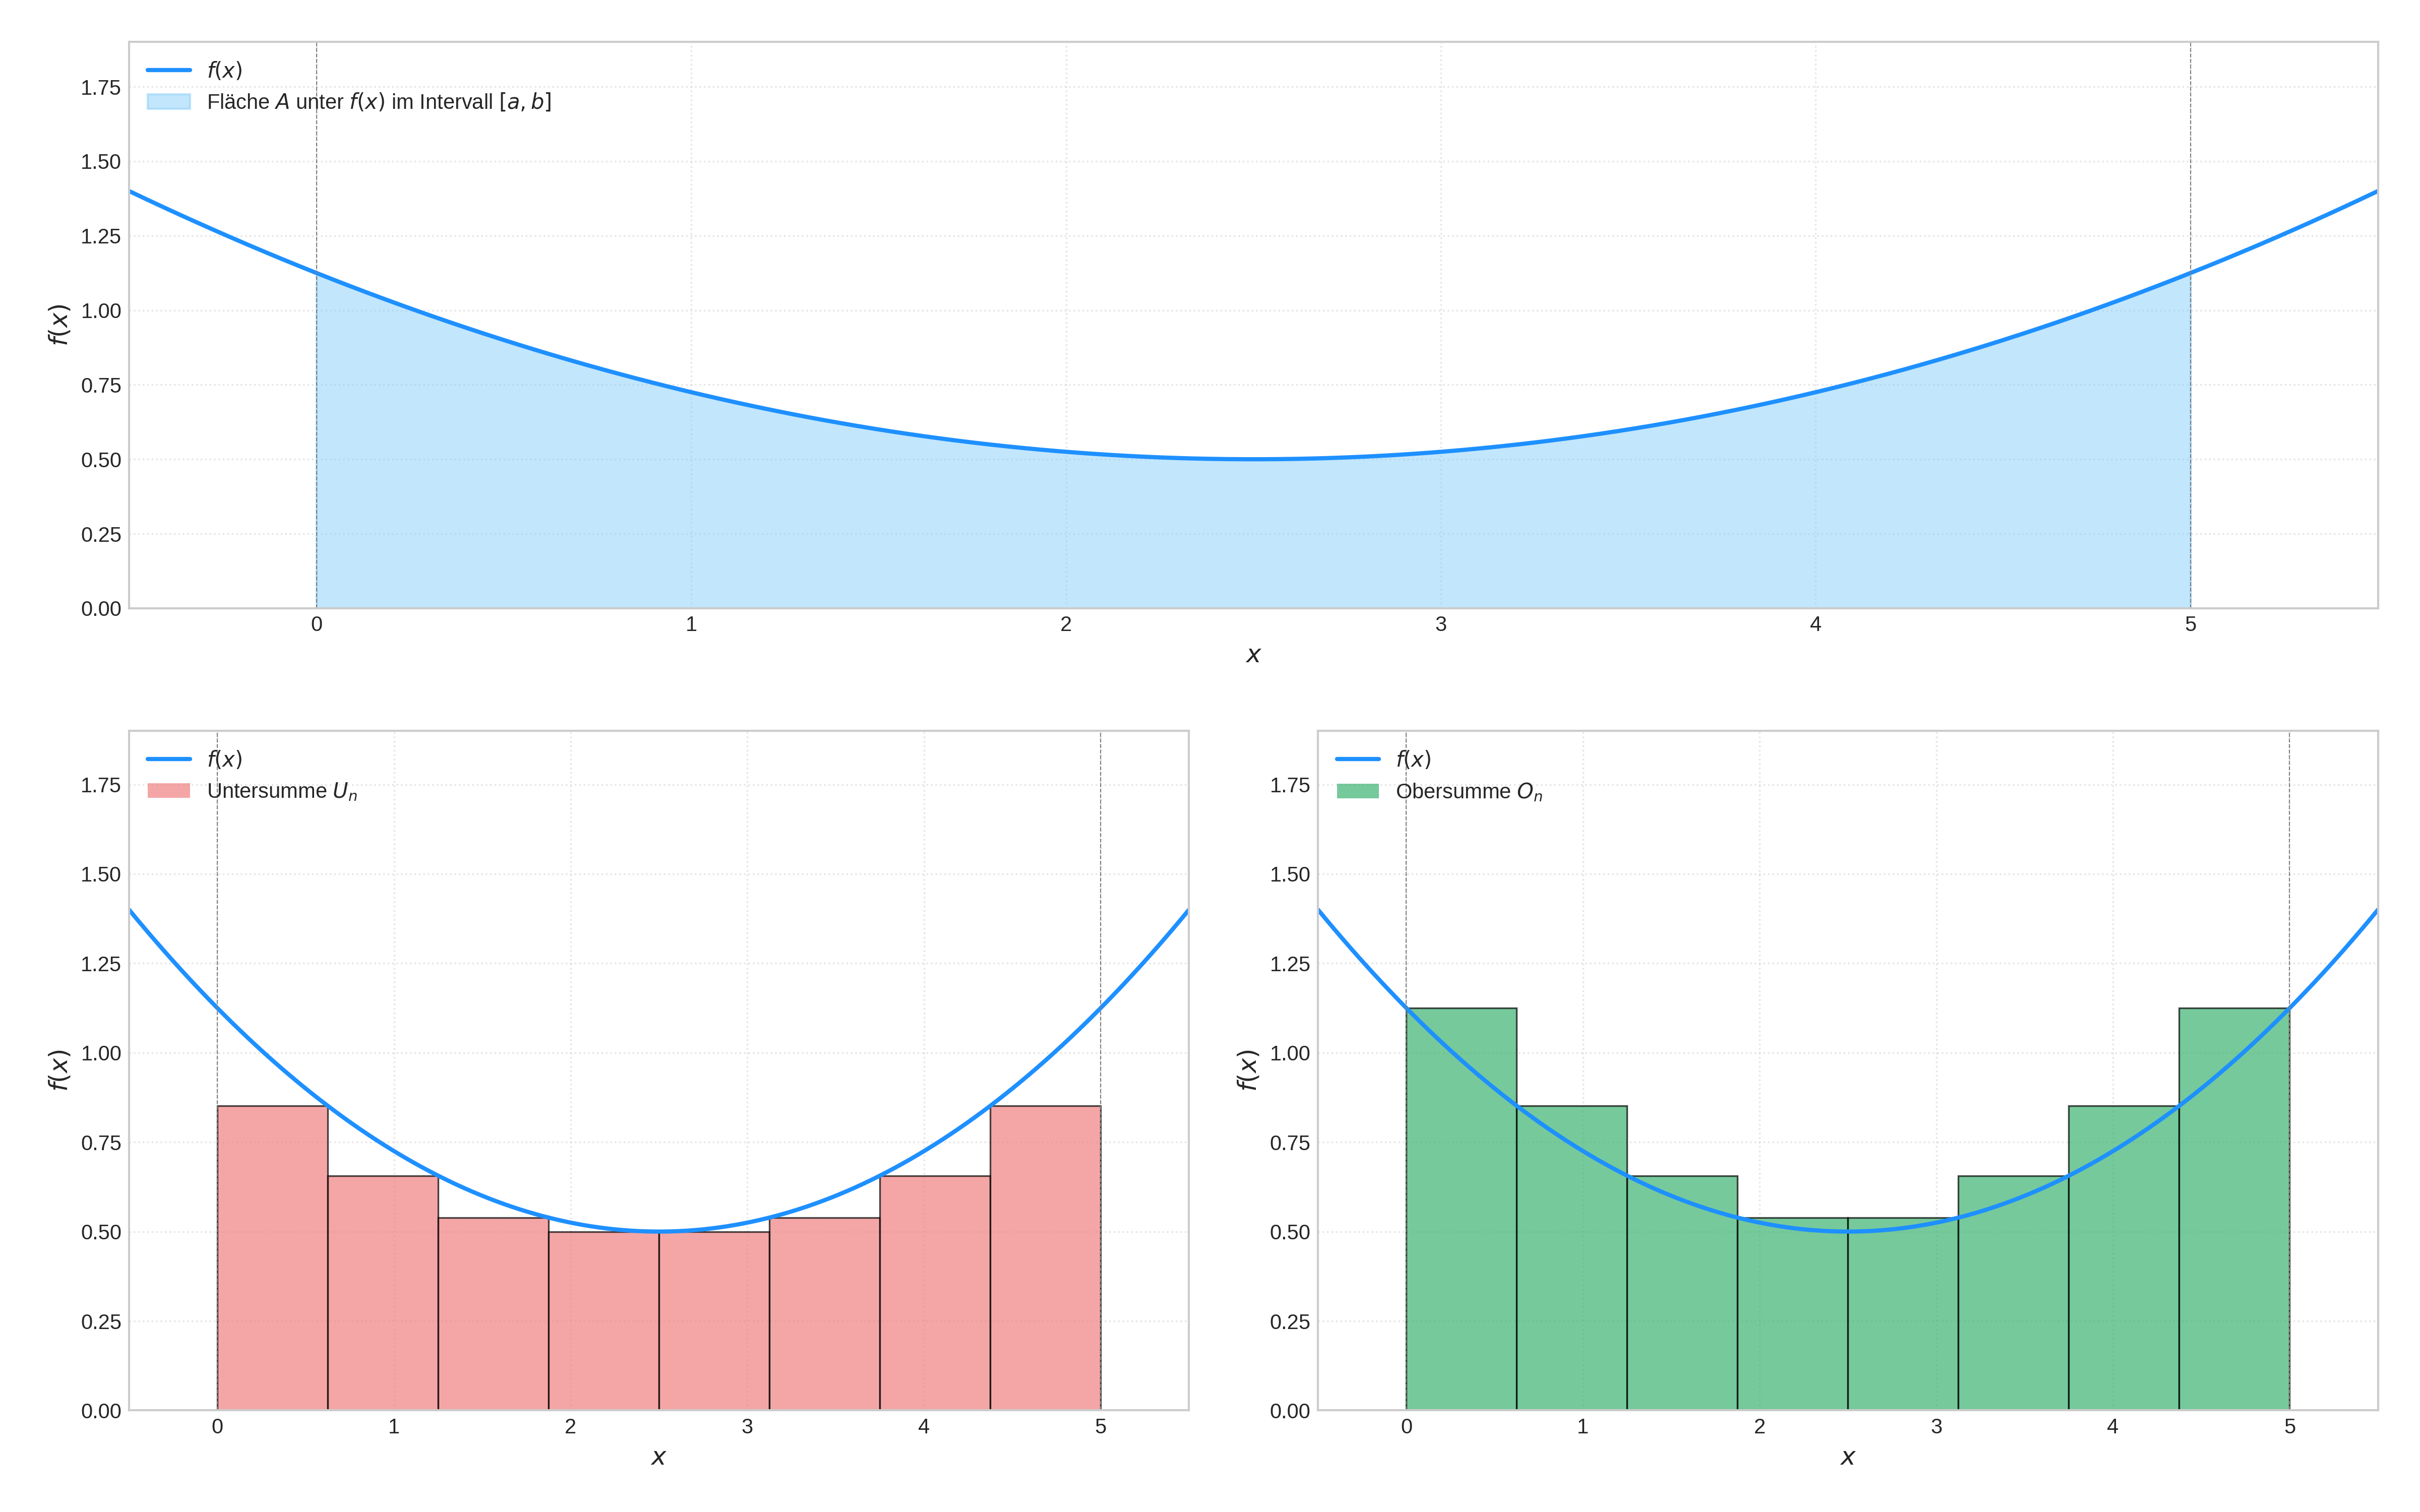
\includegraphics[width=0.9\textwidth]{grafiken/Riemannsummen_Untersumme_Obersumme.png}
    \captionof{figure}{Illustration von Untersumme und Obersumme (Riemannsummen)}
    \label{fig:riemannsummen_illustration}
\end{center}

Schauen wir uns ein konkretes Beispiel an, wie man eine Untersumme und eine Obersumme berechnet. Für einfache, monotone Funktionen ist die Bestimmung des Minimums/Maximums in einem Teilintervall einfach der Funktionswert am entsprechenden Rand.

\begin{beispielumgebung}{Untersumme und Obersumme für $f(x)=x^2$}
Wir wollen den Flächeninhalt unter der Funktion $f(x)=x^2$ im Intervall $[0,2]$ mit $n=4$ Teilintervallen durch Untersumme $U_4$ und Obersumme $O_4$ annähern.

\textbf{Schritt 1: Intervallbreite $\Delta x$ und Teilungspunkte $x_i$ bestimmen.}
Das Intervall ist $[a,b] = [0,2]$. Die Anzahl der Teilintervalle ist $n=4$.
Die Breite jedes Teilintervalls ist $\Delta x = \frac{b-a}{n} = \frac{2-0}{4} = \frac{2}{4} = 0.5$.
Die Teilungspunkte sind:
$x_0 = a = 0$
$x_1 = x_0 + \Delta x = 0 + 0.5 = 0.5$
$x_2 = x_1 + \Delta x = 0.5 + 0.5 = 1$
$x_3 = x_2 + \Delta x = 1 + 0.5 = 1.5$
$x_4 = x_3 + \Delta x = 1.5 + 0.5 = 2 (=b)$.

\textbf{Schritt 2: Untersumme $U_4$ berechnen.}
Die Funktion $f(x)=x^2$ ist im Intervall $[0,2]$ streng monoton steigend. Das bedeutet, der kleinste Funktionswert (Minimum) in jedem Teilintervall $[x_{i-1}, x_i]$ befindet sich am \textbf{linken Rand} $x_{i-1}$. Die Höhe des $i$-ten Rechtecks ist also $f(x_{i-1})$.
\begin{itemize}
    \item 1. Rechteck (Intervall $[x_0, x_1] = [0, 0.5]$): Höhe $f(x_0) = f(0) = 0^2 = 0$. Fläche $\Delta x \cdot f(0) = 0.5 \cdot 0 = 0$.
    \item 2. Rechteck (Intervall $[x_1, x_2] = [0.5, 1]$): Höhe $f(x_1) = f(0.5) = (0.5)^2 = 0.25$. Fläche $\Delta x \cdot f(0.5) = 0.5 \cdot 0.25 = 0.125$.
    \item 3. Rechteck (Intervall $[x_2, x_3] = [1, 1.5]$): Höhe $f(x_2) = f(1) = 1^2 = 1$. Fläche $\Delta x \cdot f(1) = 0.5 \cdot 1 = 0.5$.
    \item 4. Rechteck (Intervall $[x_3, x_4] = [1.5, 2]$): Höhe $f(x_3) = f(1.5) = (1.5)^2 = 2.25$. Fläche $\Delta x \cdot f(1.5) = 0.5 \cdot 2.25 = 1.125$.
\end{itemize}
Die Untersumme ist die Summe dieser Flächen:
$U_4 = 0 + 0.125 + 0.5 + 1.125 = 1.75$.

\textbf{Schritt 3: Obersumme $O_4$ berechnen.}
Da $f(x)=x^2$ im Intervall $[0,2]$ streng monoton steigend ist, liegt der größte Funktionswert (Maximum) in jedem Teilintervall $[x_{i-1}, x_i]$ am \textbf{rechten Rand} $x_i$. Die Höhe des $i$-ten Rechtecks ist also $f(x_i)$.
\begin{itemize}
    \item 1. Rechteck (Intervall $[x_0, x_1] = [0, 0.5]$): Höhe $f(x_1) = f(0.5) = (0.5)^2 = 0.25$. Fläche $\Delta x \cdot f(0.5) = 0.5 \cdot 0.25 = 0.125$.
    \item 2. Rechteck (Intervall $[x_1, x_2] = [0.5, 1]$): Höhe $f(x_2) = f(1) = 1^2 = 1$. Fläche $\Delta x \cdot f(1) = 0.5 \cdot 1 = 0.5$.
    \item 3. Rechteck (Intervall $[x_2, x_3] = [1, 1.5]$): Höhe $f(x_3) = f(1.5) = (1.5)^2 = 2.25$. Fläche $\Delta x \cdot f(1.5) = 0.5 \cdot 2.25 = 1.125$.
    \item 4. Rechteck (Intervall $[x_3, x_4] = [1.5, 2]$): Höhe $f(x_4) = f(2) = 2^2 = 4$. Fläche $\Delta x \cdot f(2) = 0.5 \cdot 4 = 2$.
\end{itemize}
Die Obersumme ist die Summe dieser Flächen:
$O_4 = 0.125 + 0.5 + 1.125 + 2 = 3.75$.

Der wahre Flächeninhalt $A$ unter $f(x)=x^2$ im Intervall $[0,2]$ liegt also zwischen $1.75$ und $3.75$:
$1.75 \le A \le 3.75$.
Wenn wir $n$ erhöhen, wird diese 'Schere' zwischen Unter- und Obersumme immer kleiner. Der exakte Wert ist übrigens $A = \frac{8}{3} \approx 2.667$. Unsere Näherungen sind also noch recht grob, aber sie zeigen das Prinzip.
\end{beispielumgebung}

\begin{tippumgebung}{Summenformel für Riemannsummen}
Allgemein lässt sich die Untersumme $U_n$ und Obersumme $O_n$ mit dem Summenzeichen $\sum$ schreiben:
Sei $m_i$ das Minimum von $f(x)$ im $i$-ten Teilintervall $[x_{i-1}, x_i]$ und $M_i$ das Maximum.
Dann ist:
\[ U_n = \sum_{i=1}^{n} m_i \cdot \Delta x \]
\[ O_n = \sum_{i=1}^{n} M_i \cdot \Delta x \]
Wenn $f(x)$ im Intervall $[a,b]$ monoton steigend ist, dann ist $m_i = f(x_{i-1})$ (linker Rand) und $M_i = f(x_i)$ (rechter Rand).
Wenn $f(x)$ im Intervall $[a,b]$ monoton fallend ist, dann ist $m_i = f(x_i)$ (rechter Rand) und $M_i = f(x_{i-1})$ (linker Rand).
\end{tippumgebung}

\begin{aufgabenumgebung}{Riemannsummen berechnen}
Gegeben ist die Funktion $f(x) = x+1$.
\begin{enumerate}
    \item Berechne die Untersumme $U_5$ und die Obersumme $O_5$ für das Intervall $[0,5]$ mit $n=5$ Teilintervallen.
    \begin{tippumgebung}{Monotonie}
    Ist $f(x)=x+1$ monoton steigend oder fallend? Wo liegt also das Minimum bzw. Maximum in jedem Teilintervall?
    \end{tippumgebung}
    \item Der Graph von $f(x)=x+1$ ist eine Gerade. Der Bereich unter dem Graphen im Intervall $[0,5]$ bildet ein Trapez. Berechne den exakten Flächeninhalt dieses Trapezes mit der geometrischen Formel $A_{Trapez} = \frac{(a+c)}{2} \cdot h$ (wobei $a$ und $c$ die parallelen Seiten sind und $h$ die Höhe).
    \item Vergleiche deine Ergebnisse für $U_5$ und $O_5$ mit dem exakten Flächeninhalt.
    \item Was würde passieren, wenn du $n=10$ oder $n=100$ Teilintervalle wählen würdest? Wie würden sich $U_n$ und $O_n$ verändern?
\end{enumerate}

\begin{center}
    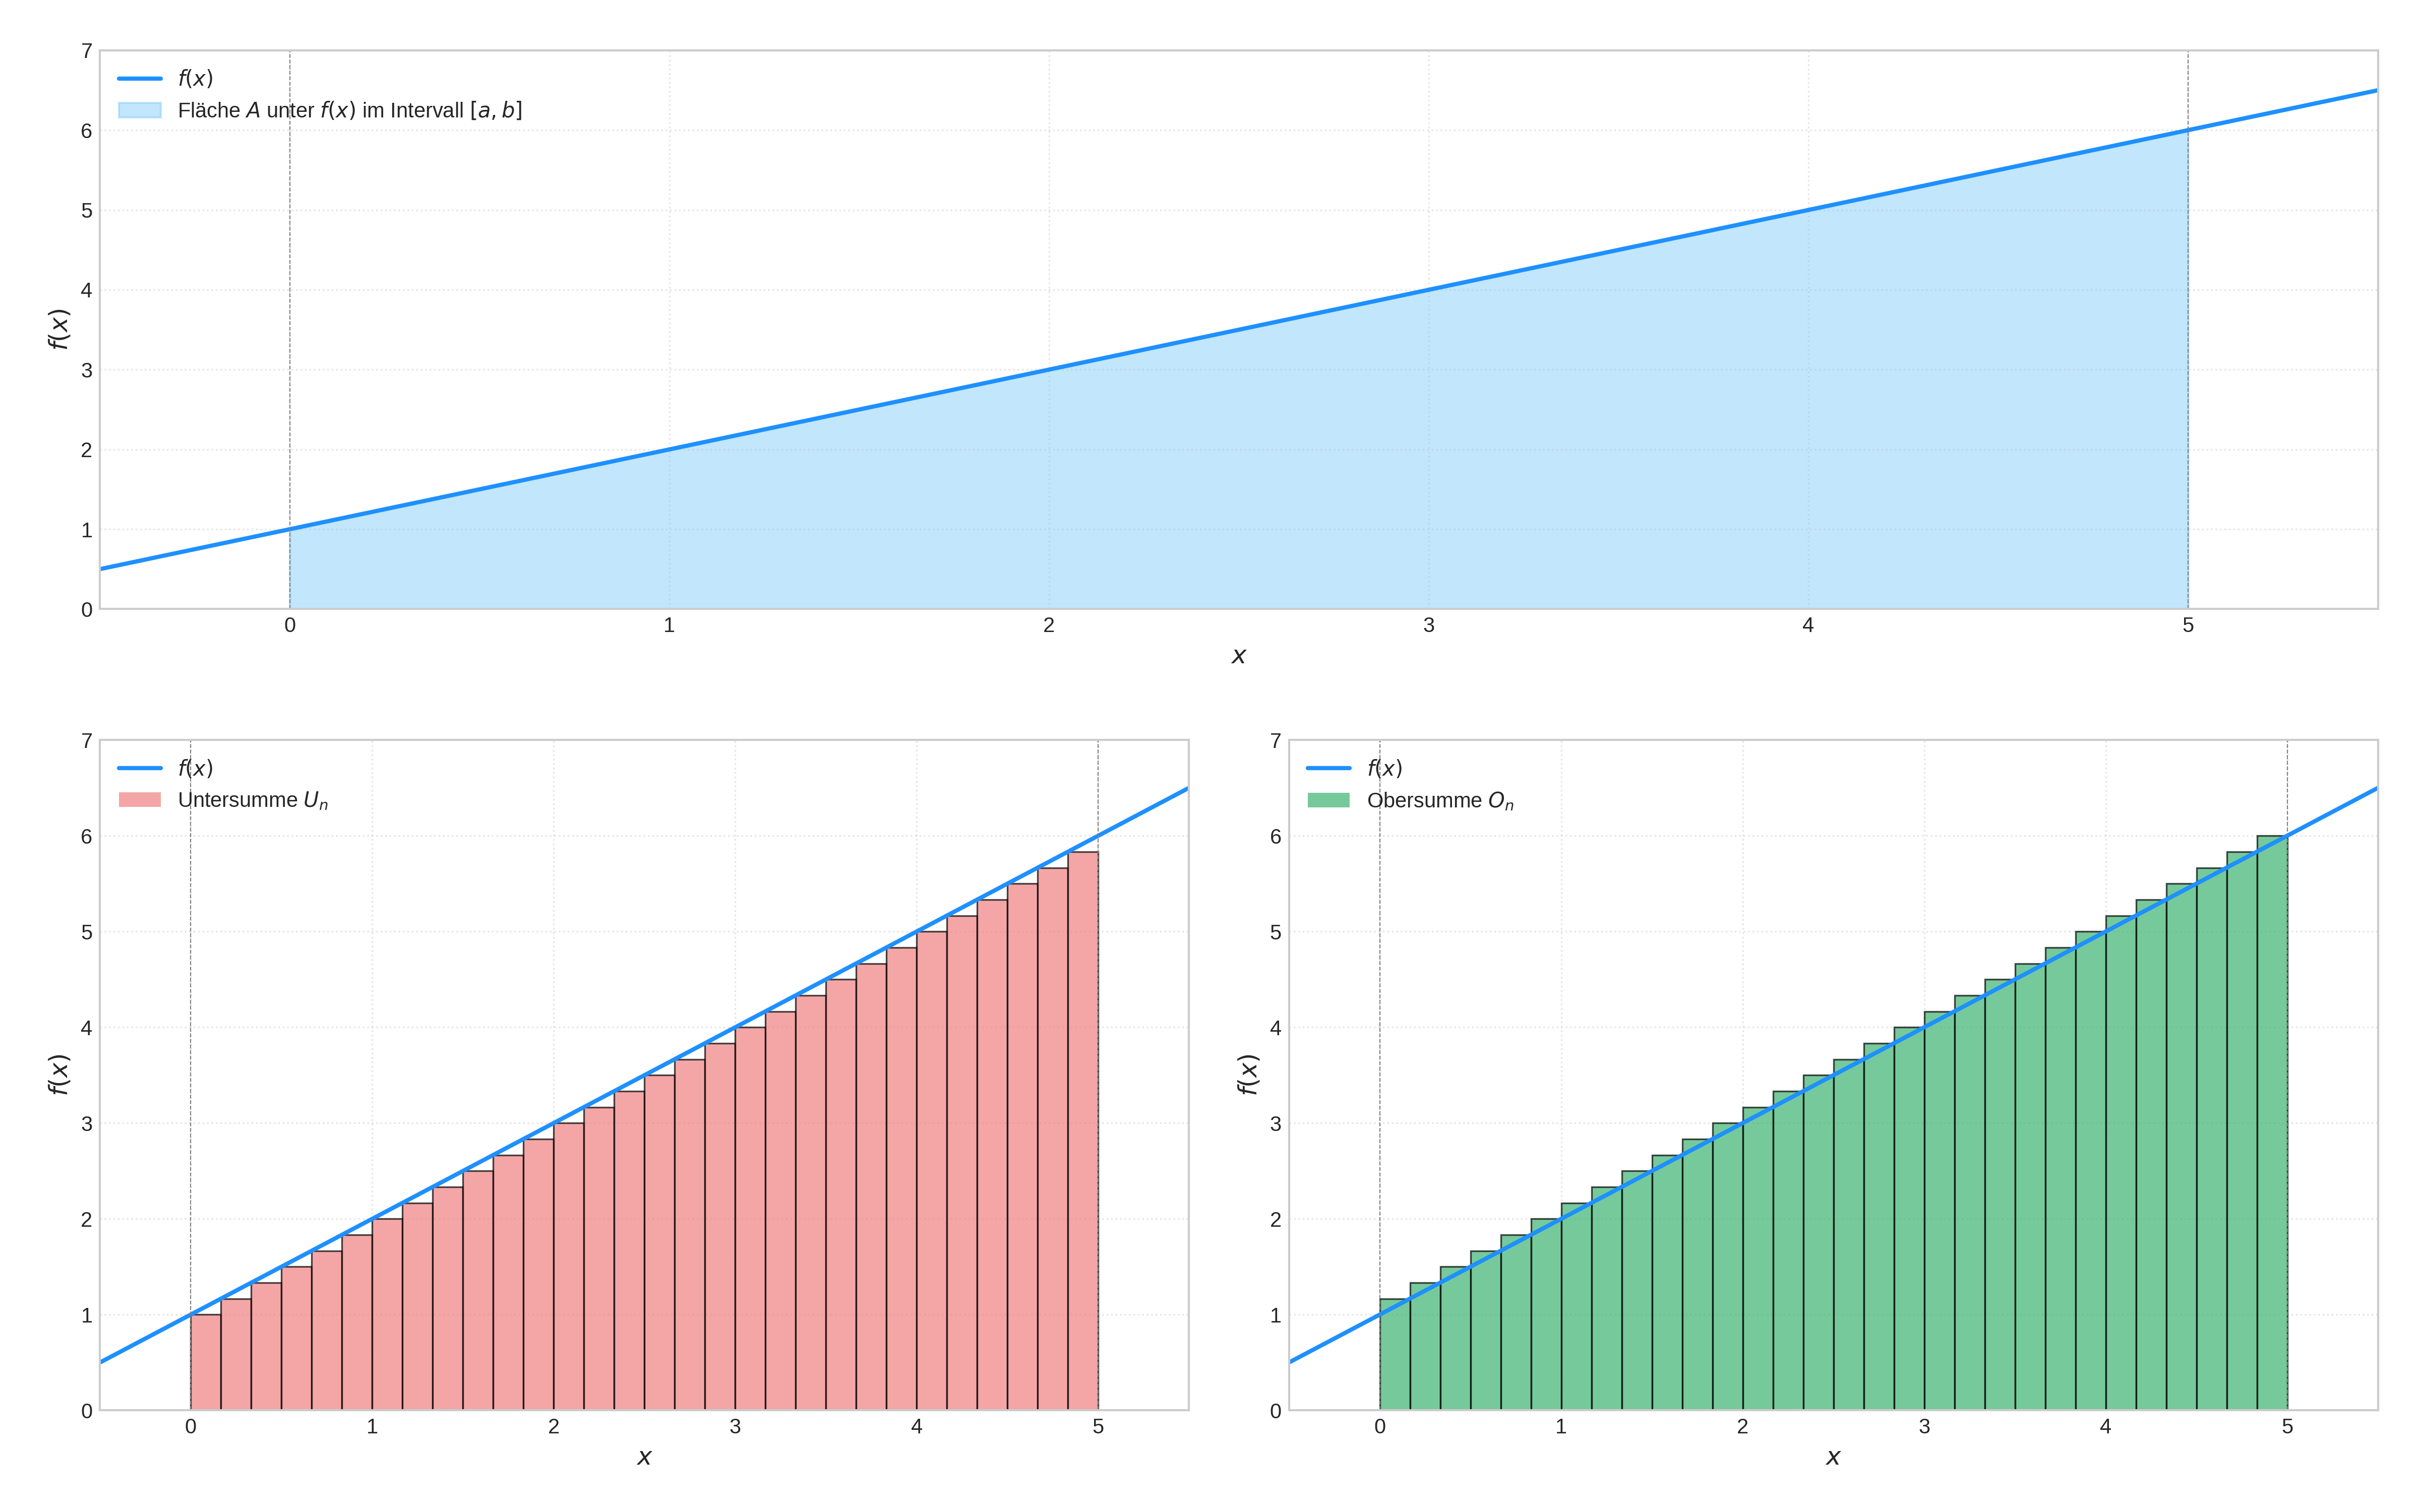
\includegraphics[width=0.9\textwidth]{grafiken/Riemannsummen_lineareFunktion.png}
    \captionof{figure}{Fläche unter $f(x)=x+1$ im Intervall $[0,5]$ }
    \label{fig:riemannsummen_linear_illustration}
\end{center}
\end{aufgabenumgebung}

Die Idee der Riemannsummen führt uns direkt zum Begriff des \textbf{bestimmten Integrals}.

\subsection{Das bestimmte Integral – Der exakte Flächeninhalt}
\label{subsec:bestimmtes_integral_neu} % Neues Label

Wir haben gesehen, dass wir den Flächeninhalt unter einer Kurve durch Riemannsummen (z.B. Unter- und Obersummen) annähern können. Je mehr Rechtecke wir verwenden (je größer $n$ wird und damit je kleiner $\Delta x = \frac{b-a}{n}$ wird), desto genauer wird unsere Näherung.

Wenn wir diesen Prozess ins Unendliche treiben, also $n \to \infty$ (und damit $\Delta x \to 0$), dann konvergieren die Untersumme und die Obersumme (für 'nette', d.h. integrierbare Funktionen) gegen denselben Wert. Dieser gemeinsame Grenzwert ist der exakte Flächeninhalt unter der Kurve und wird als das \textbf{bestimmte Integral} der Funktion $f(x)$ von $a$ bis $b$ bezeichnet.

\begin{merksatzumgebung}{Das bestimmte Integral}
Das \textbf{bestimmte Integral} einer Funktion $f(x)$ im Intervall $[a,b]$ ist der Grenzwert der Riemannsummen, wenn die Anzahl der Teilintervalle $n$ gegen unendlich geht (und die Breite $\Delta x$ der Teilintervalle gegen Null geht):
\[ \int_{a}^{b} f(x) \,dx = \lim_{n \to \infty} \sum_{i=1}^{n} f(x_i^*) \cdot \Delta x \]
Dabei ist:
\begin{itemize}
    \item $\int$ das \textbf{Integrationszeichen} (ein stilisiertes S für 'Summe').
    \item $a$ die \textbf{untere Integrationsgrenze}.
    \item $b$ die \textbf{obere Integrationsgrenze}.
    \item $f(x)$ der \textbf{Integrand} (die zu integrierende Funktion).
    \item $dx$ das \textbf{Differential}, das anzeigt, nach welcher Variablen integriert wird (hier $x$) und symbolisiert die unendlich kleine Breite der Rechtecke.
\end{itemize}
Wenn $f(x) \ge 0$ im Intervall $[a,b]$ ist, dann gibt $\int_{a}^{b} f(x) \,dx$ den \textbf{Flächeninhalt} der Fläche an, die vom Graphen von $f(x)$, der x-Achse und den senkrechten Geraden $x=a$ und $x=b$ eingeschlossen wird.
\end{merksatzumgebung}

\begin{infoboxumgebung}{Was passiert, wenn $f(x)$ unterhalb der x-Achse liegt?}
Wenn der Graph von $f(x)$ in einem Intervall unterhalb der x-Achse verläuft (also $f(x) < 0$), dann liefert das bestimmte Integral in diesem Bereich einen \textbf{negativen Wert}. Dieser negative Wert entspricht dem Flächeninhalt zwischen dem Graphen und der x-Achse, aber eben mit negativem Vorzeichen.
Man spricht dann von einer \textbf{orientierten Fläche}. Flächenanteile oberhalb der x-Achse zählen positiv, Flächenanteile unterhalb der x-Achse zählen negativ.
Um den 'echten' geometrischen Flächeninhalt zu bekommen, wenn Teile unterhalb liegen, muss man die Beträge der entsprechenden Integrale addieren oder die Funktion an den entsprechenden Stellen spiegeln (also $|f(x)|$ integrieren).
\begin{center}
    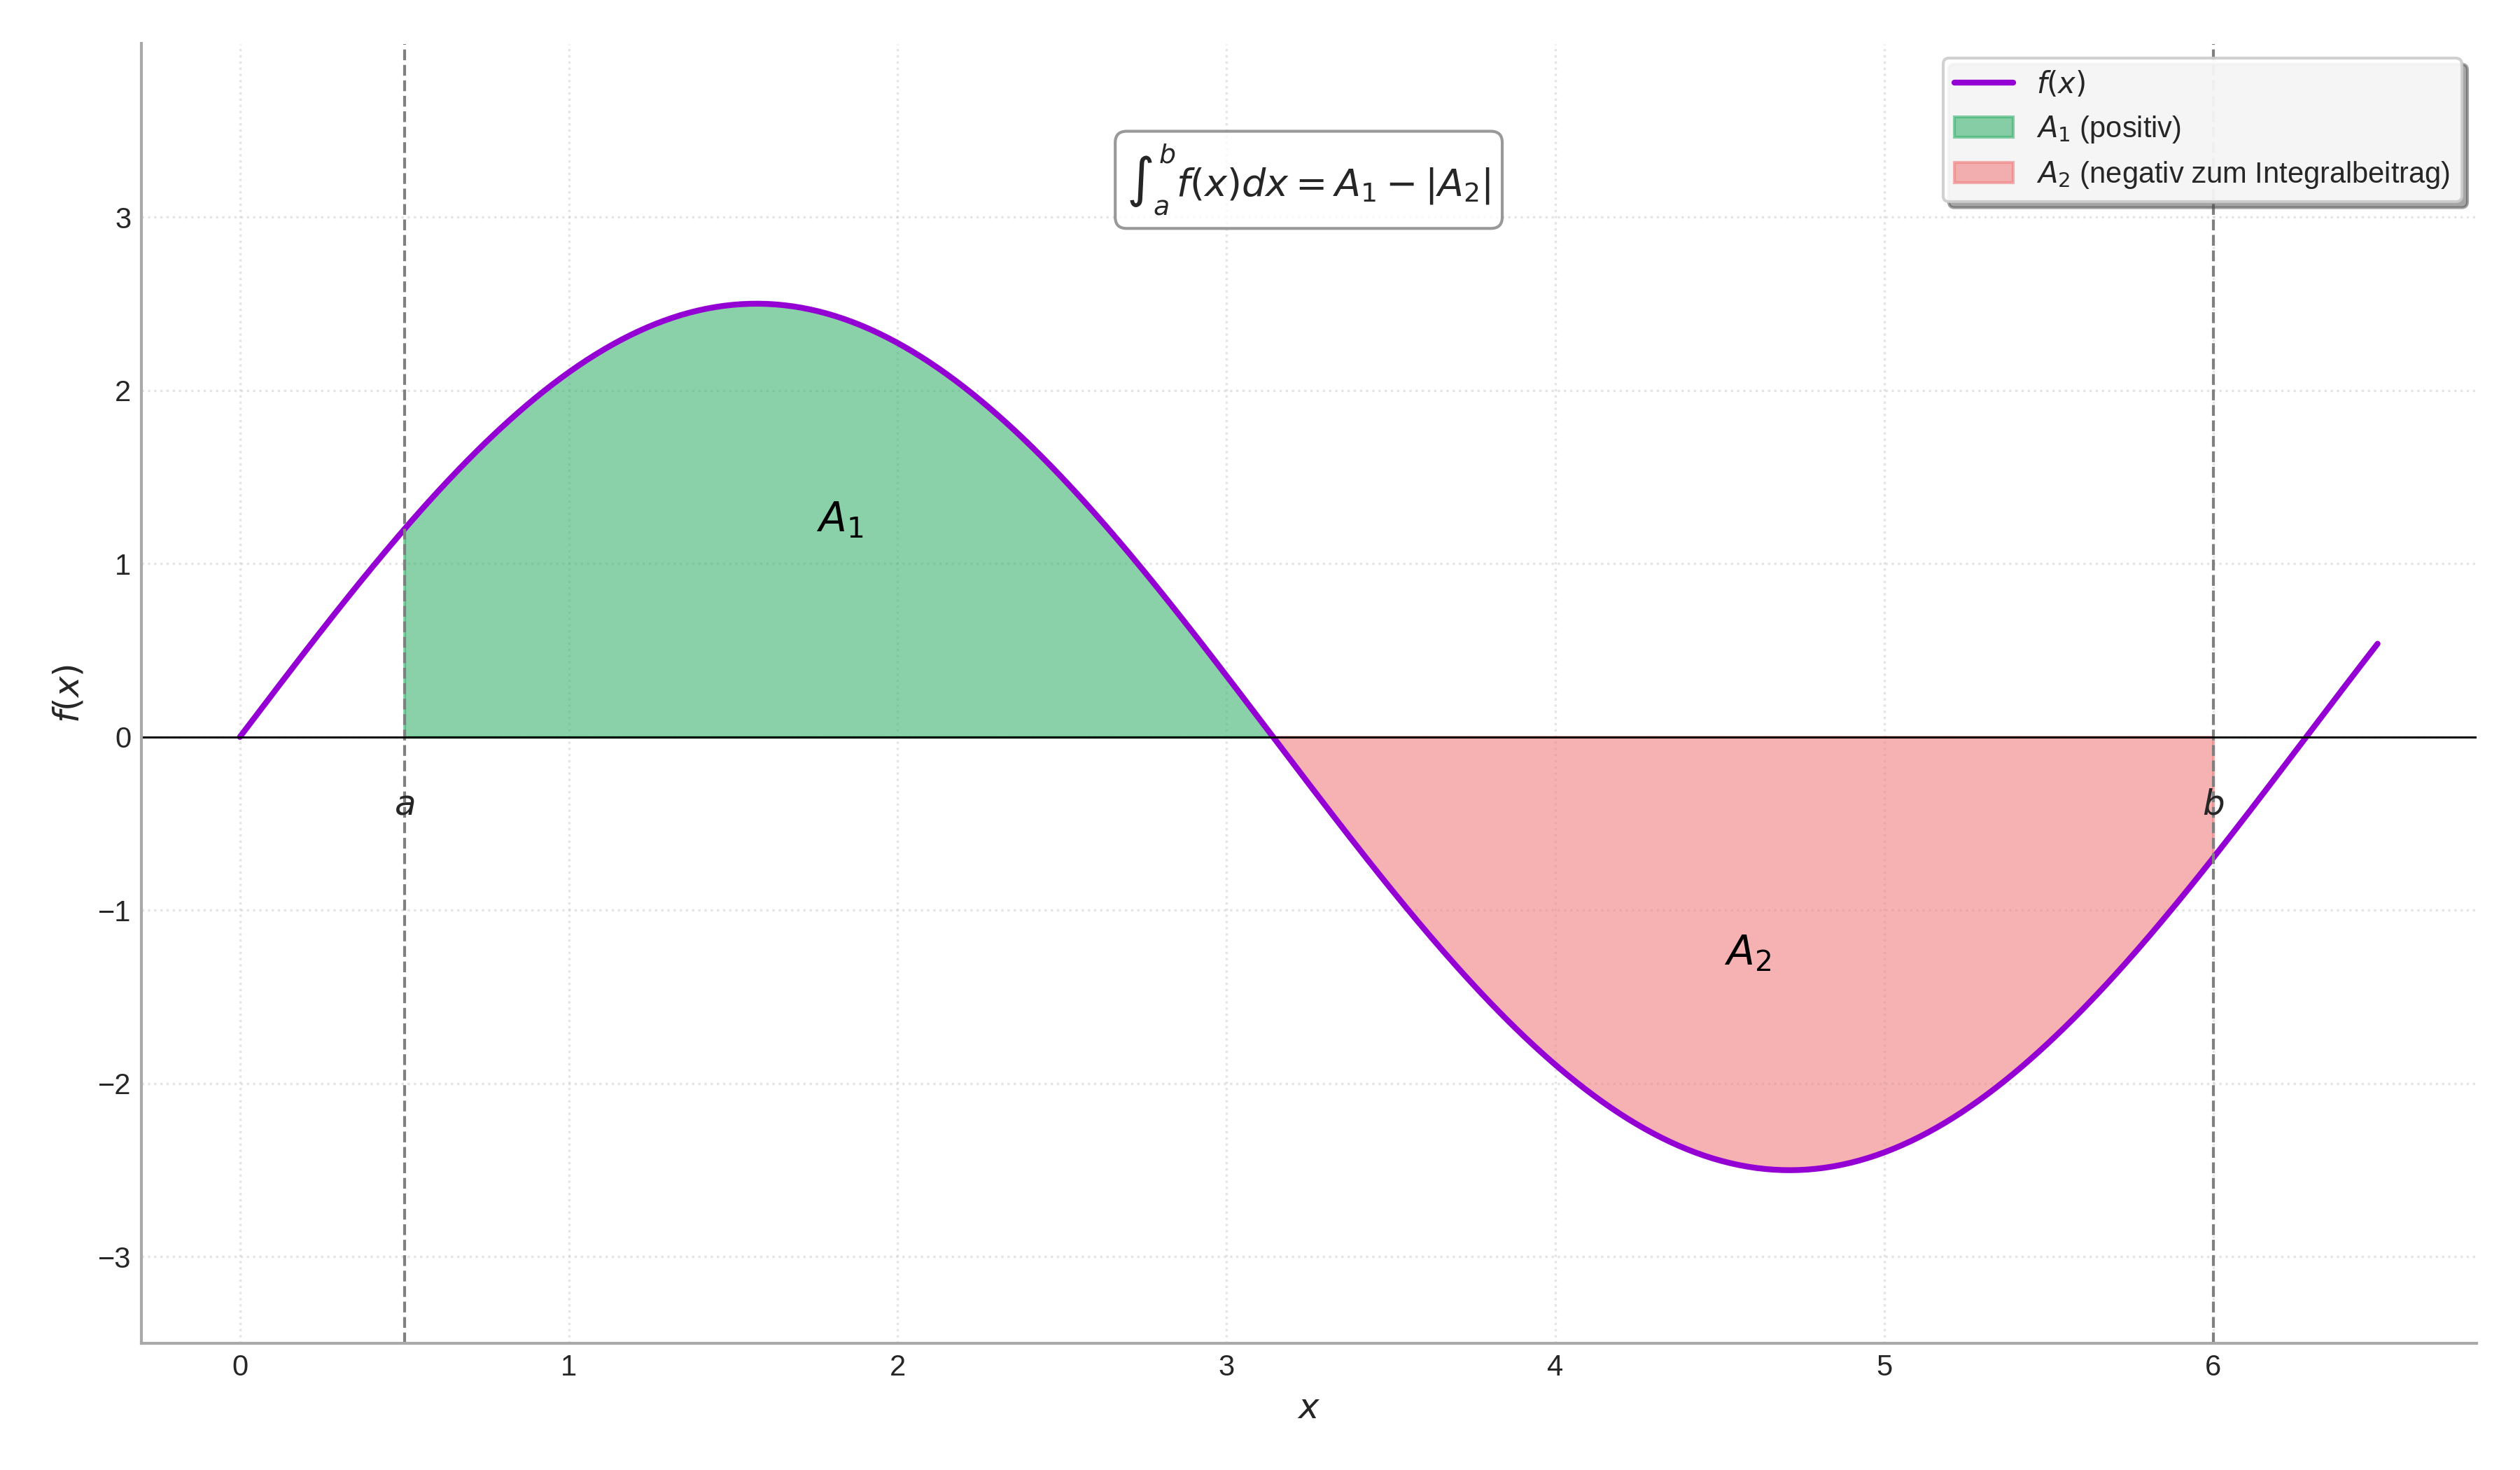
\includegraphics[width=0.8\textwidth]{grafiken/Integral_Orientierte_Flaeche.png}
    \captionof{figure}{Orientierter Flächeninhalt beim bestimmten Integral}
    \label{fig:orientierte_flaeche}
\end{center}
\end{infoboxumgebung}

\begin{fehlerboxumgebung}{Orientierte vs. geometrische Fläche – Genau hinschauen!}
Das bestimmte Integral liefert die Flächenbilanz, nicht immer den rein geometrischen Flächeninhalt!
\begin{itemize}
    \item \textbf{Orientierte Fläche:} Das Ergebnis von $\int_a^b f(x)dx$ ist die \textbf{Summe der vorzeichenbehafteten Flächenstücke}. Flächen über der x-Achse gehen positiv ein, Flächen darunter negativ.
    \item \textbf{Geometrischer Gesamtflächeninhalt gesucht?} Wenn die Aufgabe nach dem tatsächlichen, sichtbaren Flächeninhalt zwischen Graph und x-Achse fragt, musst du aufpassen:
    \begin{itemize}
        \item \textbf{Nullstellen prüfen:} Bestimme immer zuerst die Nullstellen von $f(x)$ im Intervall $[a,b]$. Diese teilen das Gesamtintervall eventuell in Teilintervalle auf.
        \item \textbf{Teilintervalle betrachten:} Untersuche das Vorzeichen von $f(x)$ in jedem Teilintervall.
        \item \textbf{Beträge addieren:} Für Teilintervalle, in denen $f(x) < 0$ (Graph unter der x-Achse), ist das Integral negativ. Für den geometrischen Flächeninhalt musst du den \textbf{Betrag} dieses negativen Wertes nehmen und zu den positiven Flächenanteilen addieren.
    \end{itemize}
    \item \textbf{Negatives Integral $\neq$ Rechenfehler:} Ein negatives Ergebnis für ein bestimmtes Integral ist oft korrekt und bedeutet lediglich, dass der Flächenanteil unterhalb der x-Achse im betrachteten Intervall überwiegt (oder die gesamte Fläche unterhalb liegt).
\end{itemize}
\end{fehlerboxumgebung}

Die Berechnung von Integralen über den Grenzwert von Riemannsummen ist sehr aufwendig. Glücklicherweise gibt es einen viel eleganteren Weg, der die Integralrechnung mit der Differentialrechnung verbindet: den Hauptsatz der Differential- und Integralrechnung. Dafür benötigen wir aber zuerst das Konzept der Stammfunktion.

\subsection{Die Stammfunktion – Das 'Gegenteil' vom Ableiten (Aufleiten)}
\label{subsec:stammfunktion_integral} % Neues Label

In der Differentialrechnung haben wir gelernt, zu einer gegebenen Funktion $f(x)$ ihre Ableitungsfunktion $f'(x)$ zu finden, die uns die Steigung von $f(x)$ an jeder Stelle liefert.
Die Integralrechnung stellt nun oft die umgekehrte Frage:
\textit{Wenn wir eine Funktion $f(x)$ gegeben haben (die wir uns jetzt als Ableitung einer anderen Funktion vorstellen können), welche Funktion $F(x)$ müssen wir ableiten, um genau dieses $f(x)$ als Ergebnis zu erhalten?}
Eine solche Funktion $F(x)$ nennen wir eine \textbf{Stammfunktion} von $f(x)$.

\begin{merksatzumgebung}{Stammfunktion}
Eine Funktion $F(x)$ heißt \textbf{Stammfunktion} einer Funktion $f(x)$, wenn für alle $x$ im Definitionsbereich gilt:
\[ F'(x) = f(x) \]
Das bedeutet, die Ableitung der Stammfunktion $F(x)$ ergibt die ursprüngliche Funktion $f(x)$.
Den Vorgang des Findens einer Stammfunktion nennt man auch \textbf{Integrieren} oder umgangssprachlich (und sehr anschaulich) \textbf{Aufleiten}.
\end{merksatzumgebung}

Das Finden von Stammfunktionen ist also wie ein Rätsel: 'Welche Funktion wurde hier abgeleitet?'

\begin{beispielumgebung}{Stammfunktionen finden durch 'Rückwärts-Ableiten'}
\begin{enumerate}
    \item \textbf{Gegeben: $f(x) = 2x$.}
        Wir fragen uns: Welche Funktion $F(x)$ hat als Ableitung $2x$?
        Aus der Potenzregel der Ableitung wissen wir: $(x^2)' = 2x^1 = 2x$.
        Also ist $F(x) = x^2$ eine Stammfunktion von $f(x)=2x$.

        \textit{Aber Moment mal!} Was ist mit $F_1(x) = x^2 + 5$?
        $F_1'(x) = (x^2)' + (5)' = 2x + 0 = 2x$.
        Auch $F_1(x) = x^2+5$ ist eine Stammfunktion von $f(x)=2x$.

        Und was ist mit $F_2(x) = x^2 - 17$?
        $F_2'(x) = (x^2)' - (17)' = 2x - 0 = 2x$.
        Ebenfalls eine Stammfunktion!

        Es scheint unendlich viele Stammfunktionen zu geben, die sich nur durch eine additive Konstante unterscheiden.

    \item \textbf{Gegeben: $f(x) = x^2$.}
        Welche Funktion $F(x)$ ergibt abgeleitet $x^2$?
        Wir wissen, beim Ableiten wird der Exponent um 1 kleiner. Also muss der Exponent der Stammfunktion um 1 größer sein, also $x^3$.
        Probieren wir $G(x)=x^3$. Die Ableitung ist $G'(x)=3x^2$.
        Das ist noch nicht ganz $x^2$, sondern das Dreifache. Um das auszugleichen, müssen wir $x^3$ durch 3 teilen:
        $F(x) = \frac{1}{3}x^3$.
        Machen wir die Probe: $F'(x) = (\frac{1}{3}x^3)' = \frac{1}{3} \cdot (3x^2) = x^2$. Perfekt!
        Also ist $F(x) = \frac{1}{3}x^3$ eine Stammfunktion von $f(x)=x^2$.
        Und natürlich sind auch $F(x) = \frac{1}{3}x^3 + 7$ oder $F(x) = \frac{1}{3}x^3 - \pi$ Stammfunktionen.
\end{enumerate}
\end{beispielumgebung}

Das erste Beispiel hat uns eine wichtige Eigenschaft gezeigt:

\begin{merksatzumgebung}{Die Menge aller Stammfunktionen (Das unbestimmte Integral)}
Wenn $F(x)$ eine Stammfunktion einer Funktion $f(x)$ ist (d.h. $F'(x)=f(x)$), dann ist auch jede Funktion der Form $F(x)+C$, wobei $C$ eine beliebige reelle Konstante ist, eine Stammfunktion von $f(x)$.
Denn $(F(x)+C)' = F'(x) + (C)' = f(x) + 0 = f(x)$.

Die Menge aller dieser Stammfunktionen wird als das \textbf{unbestimmte Integral} von $f(x)$ bezeichnet und man schreibt dafür:
\[ \int f(x) \,dx = F(x) + C \]
Dabei ist:
\begin{itemize}
    \item $\int$ das \textbf{Integrationszeichen} (ein stilisiertes S, das an 'Summe' erinnert – ein Hinweis auf die Riemannsummen, die wir später kennenlernen).
    \item $f(x)$ der \textbf{Integrand} (die Funktion, die integriert/aufgeleitet wird).
    \item $dx$ das \textbf{Differential}, das anzeigt, nach welcher Variablen integriert wird (hier $x$). Es ist ein wichtiger Bestandteil der Notation.
    \item $F(x)$ irgendeine spezielle Stammfunktion von $f(x)$.
    \item $C$ die \textbf{Integrationskonstante} (eine beliebige reelle Zahl).
\end{itemize}
Das unbestimmte Integral liefert uns also nicht nur eine einzelne Funktion, sondern eine ganze \textbf{Schar von Funktionen}, die sich alle nur durch eine Verschiebung entlang der y-Achse unterscheiden.
\end{merksatzumgebung}

\textit{Selbst-Check:} Warum ist es wichtig, die Integrationskonstante $C$ beim unbestimmten Integral anzugeben? (Antwort: Weil es unendlich viele Funktionen gibt, deren Ableitung $f(x)$ ist, und $C$ repräsentiert all diese Möglichkeiten.)

\subsubsection{Grundlegende Integrationsregeln (Umkehrung der Ableitungsregeln)}
Ähnlich wie beim Ableiten gibt es auch beim Integrieren Regeln, die uns helfen, Stammfunktionen systematisch zu finden. Viele davon ergeben sich direkt durch Umkehrung der uns bekannten Ableitungsregeln. Wir konzentrieren uns hier zunächst auf Regeln für Polynomfunktionen.

\begin{merksatzumgebung}{Grundlegende Integrationsregeln für Polynome}
\begin{itemize}
    \item \textbf{Potenzregel der Integration:} Für $f(x) = x^n$ (mit $n \in \mathbb{R}, n \neq -1$) gilt:
    \[ \int x^n \,dx = \frac{1}{n+1}x^{n+1} + C \]
    \textit{Regel in Worten:} 'Erhöhe den Exponenten um 1 und teile dann durch diesen neuen Exponenten.'
    \textit{Beachte:} Diese Regel gilt nicht für $n=-1$, also für $f(x)=x^{-1}=\frac{1}{x}$. Die Stammfunktion von $\frac{1}{x}$ ist $\ln|x|+C$. Dies werden wir später bei den Logarithmusfunktionen genauer betrachten. Für Polynome tritt dieser Fall aber nicht auf.

    \item \textbf{Faktorregel der Integration:} Ein konstanter Faktor $k$ kann vor das Integral gezogen werden:
    \[ \int k \cdot f(x) \,dx = k \cdot \int f(x) \,dx \]
    Das bedeutet, wir können erst die Stammfunktion von $f(x)$ finden und diese dann mit $k$ multiplizieren.

    \item \textbf{Summenregel der Integration:} Das Integral einer Summe (oder Differenz) von Funktionen ist die Summe (oder Differenz) ihrer Integrale:
    \[ \int (f(x) \pm g(x)) \,dx = \int f(x) \,dx \pm \int g(x) \,dx \]
    \textit{Regel in Worten:} 'Jeder Summand wird für sich integriert/aufgeleitet, und die Ergebnisse werden dann addiert bzw. subtrahiert.'

    \item \textbf{Integral einer Konstanten:} Für $f(x)=k$ (eine Konstante) gilt:
    \[ \int k \,dx = kx + C \]
    (Denn die Ableitung von $kx+C$ ist $k$.)
\end{itemize}
\end{merksatzumgebung}

\begin{beispielumgebung}{Stammfunktionen mit Regeln bilden}
\begin{enumerate}
    \item \textbf{Bestimme $\int x^4 \,dx$.}
        Hier ist $n=4$. Nach der Potenzregel der Integration:
        $\int x^4 \,dx = \frac{1}{4+1}x^{4+1} + C = \frac{1}{5}x^5 + C$.
        \textit{Probe durch Ableiten:} $(\frac{1}{5}x^5+C)' = \frac{1}{5} \cdot 5x^4 + 0 = x^4$. Stimmt.

    \item \textbf{Bestimme $\int 6x^2 \,dx$.}
        Nach Faktor- und Potenzregel:
        $\int 6x^2 \,dx = 6 \cdot \int x^2 \,dx = 6 \cdot \left(\frac{1}{2+1}x^{2+1}\right) + C = 6 \cdot \frac{1}{3}x^3 + C = 2x^3 + C$.
        \textit{Probe:} $(2x^3+C)' = 2 \cdot 3x^2 + 0 = 6x^2$. Stimmt.

    \item \textbf{Bestimme $\int (3x^2 - 4x + 5) \,dx$.}
        Nach Summen-, Faktor- und Potenzregel:
        $\int (3x^2 - 4x + 5) \,dx = \int 3x^2 \,dx - \int 4x \,dx + \int 5 \,dx$
        $= 3 \cdot \int x^2 \,dx - 4 \cdot \int x^1 \,dx + \int 5x^0 \,dx$
        $= 3 \cdot \left(\frac{1}{3}x^3\right) - 4 \cdot \left(\frac{1}{2}x^2\right) + 5 \cdot \left(\frac{1}{1}x^1\right) + C$
        $= x^3 - 2x^2 + 5x + C$.
        \textit{Probe:} $(x^3 - 2x^2 + 5x + C)' = 3x^2 - 4x + 5$. Stimmt.
\end{enumerate}
\end{beispielumgebung}

\begin{aufgabenumgebung}{Stammfunktionen bilden üben}
Bestimme jeweils die Menge aller Stammfunktionen (das unbestimmte Integral) für die folgenden Funktionen:
\begin{enumerate}
    \item $f(x) = x^5$
    \item $g(x) = 12x^3$
    \item $h(x) = 2x^3 - 7x^2 + 4x - 1$
    \item $k(x) = \sqrt{x} + \frac{1}{x^3}$ (Tipp: Erst in Potenzschreibweise $x^n$ umwandeln! $\sqrt{x}=x^{1/2}$ und $\frac{1}{x^3}=x^{-3}$)
    \item $m(t) = at+b$ (wobei $a,b$ Konstanten sind; integriere nach $t$)
    \item $p(x) = (x+1)(x-2)$ (Tipp: Erst ausmultiplizieren!)
\end{enumerate}
Mache bei mindestens zwei Aufgaben die Probe durch Ableiten deiner Stammfunktion.
\end{aufgabenumgebung}

\begin{fehlerboxumgebung}{Integrationskonstante $C$ nicht vergessen!}
Ein sehr häufiger Fehler beim unbestimmten Integrieren ist das Vergessen der Integrationskonstante $+C$. Da die Ableitung einer Konstanten immer Null ist, gibt es zu jeder Funktion unendlich viele Stammfunktionen, die sich alle nur durch diese Konstante unterscheiden. Bei bestimmten Integralen (mit Grenzen) fällt diese Konstante später heraus, aber beim unbestimmten Integral ist sie wichtig! Stell dir vor, jede Stammfunktion ist wie ein Mitglied einer großen Familie von Kurven, die alle parallel zueinander verlaufen.
\end{fehlerboxumgebung}

\begin{warumwichtigumgebung}{Stammfunktionen und das unbestimmte Integral}
Das Konzept der Stammfunktion ist der Schlüssel, um den fundamentalen Zusammenhang zwischen Differential- und Integralrechnung zu verstehen. Es erlaubt uns, von einer gegebenen Änderungsrate auf die ursprüngliche Größe zurückzuschließen. Das unbestimmte Integral gibt uns die Gesamtheit aller möglichen Funktionen an, deren Ableitung die gegebene Funktion ist. Diese 'Familie' von Stammfunktionen wird entscheidend sein, wenn wir uns gleich dem bestimmten Integral und dem Hauptsatz zuwenden.
\end{warumwichtigumgebung}

Als Nächstes werden wir sehen, wie die Stammfunktion uns auf elegante Weise hilft, bestimmte Integrale und damit Flächeninhalte zu berechnen, ohne den mühsamen Weg über Riemannsummen gehen zu müssen. Das ist die Kernaussage des Hauptsatzes der Differential- und Integralrechnung.

% Vorheriger Inhalt des Kapitels bis zur warumwichtigumgebung 'Stammfunktionen und das unbestimmte Integral'
% ... (siehe vorherige Canvas-Version) ...

% Hier geht es dann weiter mit dem Hauptsatz der Differential- und Integralrechnung.
% Dieser Kommentar wird durch den folgenden Inhalt ersetzt:

\subsection{Der Hauptsatz der Differential- und Integralrechnung (HDI)}
\label{subsec:hdi}

Wir haben gesehen, dass das Berechnen von Flächeninhalten über den Grenzwert von Riemannsummen ziemlich mühsam sein kann. Gibt es einen einfacheren Weg, um das bestimmte Integral $\int_a^b f(x) \,dx$ exakt zu berechnen, ohne unendlich viele Rechtecke addieren zu müssen? Die Antwort ist ein klares Ja, und sie liegt in einem der wichtigsten Sätze der gesamten Mathematik: dem \textbf{Hauptsatz der Differential- und Integralrechnung} (oft abgekürzt als HDI).

Dieser Satz stellt eine fundamentale Verbindung zwischen der Differentialrechnung (dem Ableiten) und der Integralrechnung (dem Aufleiten bzw. Flächenberechnen) her. Er ist so etwas wie die 'magische Brücke' zwischen diesen beiden großen Gebieten der Analysis.

\begin{merksatzumgebung}{Der Hauptsatz der Differential- und Integralrechnung (HDI)}
Sei $f(x)$ eine im Intervall $[a,b]$ stetige Funktion und $F(x)$ eine beliebige Stammfunktion von $f(x)$ (d.h. $F'(x) = f(x)$). Dann gilt für das bestimmte Integral von $f(x)$ über dem Intervall $[a,b]$:
\[ \int_{a}^{b} f(x) \,dx = [F(x)]_{a}^{b} = F(b) - F(a) \]
\textbf{In Worten:} Um das bestimmte Integral von $f(x)$ in den Grenzen von $a$ bis $b$ zu berechnen, bilde eine Stammfunktion $F(x)$ von $f(x)$, setze die obere Grenze $b$ in $F(x)$ ein, setze die untere Grenze $a$ in $F(x)$ ein und subtrahiere den zweiten Wert vom ersten.

Die Schreibweise $[F(x)]_{a}^{b}$ ist eine Kurzform für $F(b) - F(a)$.
\end{merksatzumgebung}

\begin{warumwichtigumgebung}{Die Bedeutung des HDI}
Der Hauptsatz ist revolutionär, weil er uns sagt: Statt komplizierte Grenzwerte von Summen zu berechnen, um eine Fläche zu finden, können wir einfach eine Stammfunktion suchen (was oft viel einfacher ist) und deren Werte an den Rändern des Intervalls auswerten! Das Ableiten und Integrieren sind also tatsächlich Umkehroperationen zueinander.
\end{warumwichtigumgebung}

Schauen wir uns an, wie man den HDI anwendet.

\begin{beispielumgebung}{Bestimmtes Integral mit dem HDI berechnen}
\begin{enumerate}
    \item \textbf{Fläche unter $f(x)=x^2$ im Intervall $[0,2]$} (Vergleiche mit dem Riemannsummen-Beispiel!)
        Wir wollen $\int_{0}^{2} x^2 \,dx$ berechnen.
        \begin{itemize}
            \item \textbf{Schritt 1: Stammfunktion $F(x)$ von $f(x)=x^2$ finden.}
            Mit der Potenzregel der Integration: $F(x) = \frac{1}{2+1}x^{2+1} = \frac{1}{3}x^3$. (Die Integrationskonstante $C$ können wir hier weglassen, da sie sich bei der Differenz $F(b)-F(a)$ ohnehin aufheben würde: $(F(b)+C) - (F(a)+C) = F(b)-F(a)$.)
            \item \textbf{Schritt 2: Grenzen einsetzen $F(b)-F(a)$.}
            Hier ist $a=0$ und $b=2$.
            $\int_{0}^{2} x^2 \,dx = [ \frac{1}{3}x^3 ]_{0}^{2} = F(2) - F(0)$
            $= \left(\frac{1}{3}(2)^3\right) - \left(\frac{1}{3}(0)^3\right)$
            $= \frac{1}{3} \cdot 8 - \frac{1}{3} \cdot 0 = \frac{8}{3} - 0 = \frac{8}{3}$.
        \end{itemize}
        Der exakte Flächeninhalt ist $\frac{8}{3} \approx 2.667$. Das passt viel besser zu unseren Riemannsummen-Näherungen ($U_4=1.75, O_4=3.75$) und war viel einfacher zu berechnen!

    \item \textbf{Berechne $\int_{1}^{3} (3x^2 - 4x + 5) \,dx$.}
        Der Integrand ist $f(x) = 3x^2 - 4x + 5$.
        \begin{itemize}
            \item \textbf{Schritt 1: Stammfunktion $F(x)$ finden.}
            $F(x) = x^3 - 2x^2 + 5x$. (Wir lassen $C$ weg.)
            \item \textbf{Schritt 2: Grenzen einsetzen.}
            $\int_{1}^{3} (3x^2 - 4x + 5) \,dx = [x^3 - 2x^2 + 5x]_{1}^{3}$
            $= F(3) - F(1)$
            $= ((3)^3 - 2(3)^2 + 5(3)) - ((1)^3 - 2(1)^2 + 5(1))$
            $= (27 - 2 \cdot 9 + 15) - (1 - 2 \cdot 1 + 5)$
            $= (27 - 18 + 15) - (1 - 2 + 5)$
            $= (9 + 15) - (4) = 24 - 4 = 20$.
        \end{itemize}
        Der Wert des bestimmten Integrals ist 20.
\end{enumerate}
\end{beispielumgebung}

\begin{fehlerboxumgebung}{Hauptsatz-Anwendung – Typische Stolpersteine}
Der Hauptsatz der Differential- und Integralrechnung (HDI) ist mächtig, aber bei der Anwendung lauern ein paar typische Fehlerquellen:
\begin{itemize}
    \item \textbf{Grenzen vertauscht ($F(a)-F(b)$ statt $F(b)-F(a)$):} Achte penibel auf die Reihenfolge: Immer 'Stammfunktion an der oberen Grenze' minus 'Stammfunktion an der unteren Grenze', also $F(b)-F(a)$. Ein Vertauschen führt zum Vorzeichenfehler im Ergebnis!
    \item \textbf{Rechenfehler beim Einsetzen der Grenzen:} Das ist eine der häufigsten Fehlerquellen!
    \begin{itemize}
        \item Besonders bei negativen Zahlen als Grenzen oder in der Stammfunktion: Setze sorgfältig Klammern, z.B. $F(-2) = \frac{1}{3}(-2)^3 - (-2) = -\frac{8}{3} + 2$.
        \item Brüche und Potenzen korrekt berechnen. Nimm dir Zeit für diesen Schritt.
    \end{itemize}
    \item \textbf{Stammfunktion $F(x)$ falsch gebildet:} Der HDI funktioniert nur, wenn $F(x)$ auch wirklich eine korrekte Stammfunktion von $f(x)$ ist. Überprüfe deine Integrationsregeln (Potenzregel, Faktorregel, Summenregel etc.) sorgfältig. Im Zweifel: Leite deine gefundene Stammfunktion $F(x)$ zur Probe ab – es muss wieder $f(x)$ herauskommen!
    \item \textbf{Integrationskonstante $C$ beim bestimmten Integral:} Für die Berechnung des bestimmten Integrals $\int_a^b f(x)dx = F(b)-F(a)$ kannst du die Integrationskonstante $C$ weglassen (oder $C=0$ setzen), da sie sich ohnehin herauskürzen würde: $(F(b)+C) - (F(a)+C) = F(b)-F(a)$. Wenn du sie mitschleppst, achte darauf, dass sie sich korrekt aufhebt.
\end{itemize}
Sorgfältiges und schrittweises Rechnen hilft, diese Fehler zu vermeiden!
\end{fehlerboxumgebung}

\begin{aufgabenumgebung}{Bestimmte Integrale mit dem HDI berechnen}
Berechne die folgenden bestimmten Integrale mit dem Hauptsatz.
\begin{enumerate}
    \item $\int_{1}^{2} (4x^3 - 6x) \,dx$
    \item $\int_{-1}^{1} (x^2 + 2) \,dx$
    \item $\int_{0}^{4} (\sqrt{x} + 1) \,dx$ (Tipp: $\sqrt{x} = x^{1/2}$)
    \item \textbf{Fläche visualisieren:}
        Die Funktion $f(x) = -x^2 + 4x$ hast du vielleicht schon in früheren Aufgaben skizziert (eine nach unten geöffnete Parabel).
        \begin{itemize}
            \item Berechne die Nullstellen von $f(x)$.
            \item Berechne das bestimmte Integral $\int_{x_1}^{x_2} f(x) \,dx$, wobei $x_1$ und $x_2$ die Nullstellen sind ($x_1 < x_2$).
            \item Was stellt dieser Wert geometrisch dar? Markiere die entsprechende Fläche in einer Skizze des Graphen von $f(x)$.
\begin{center}
    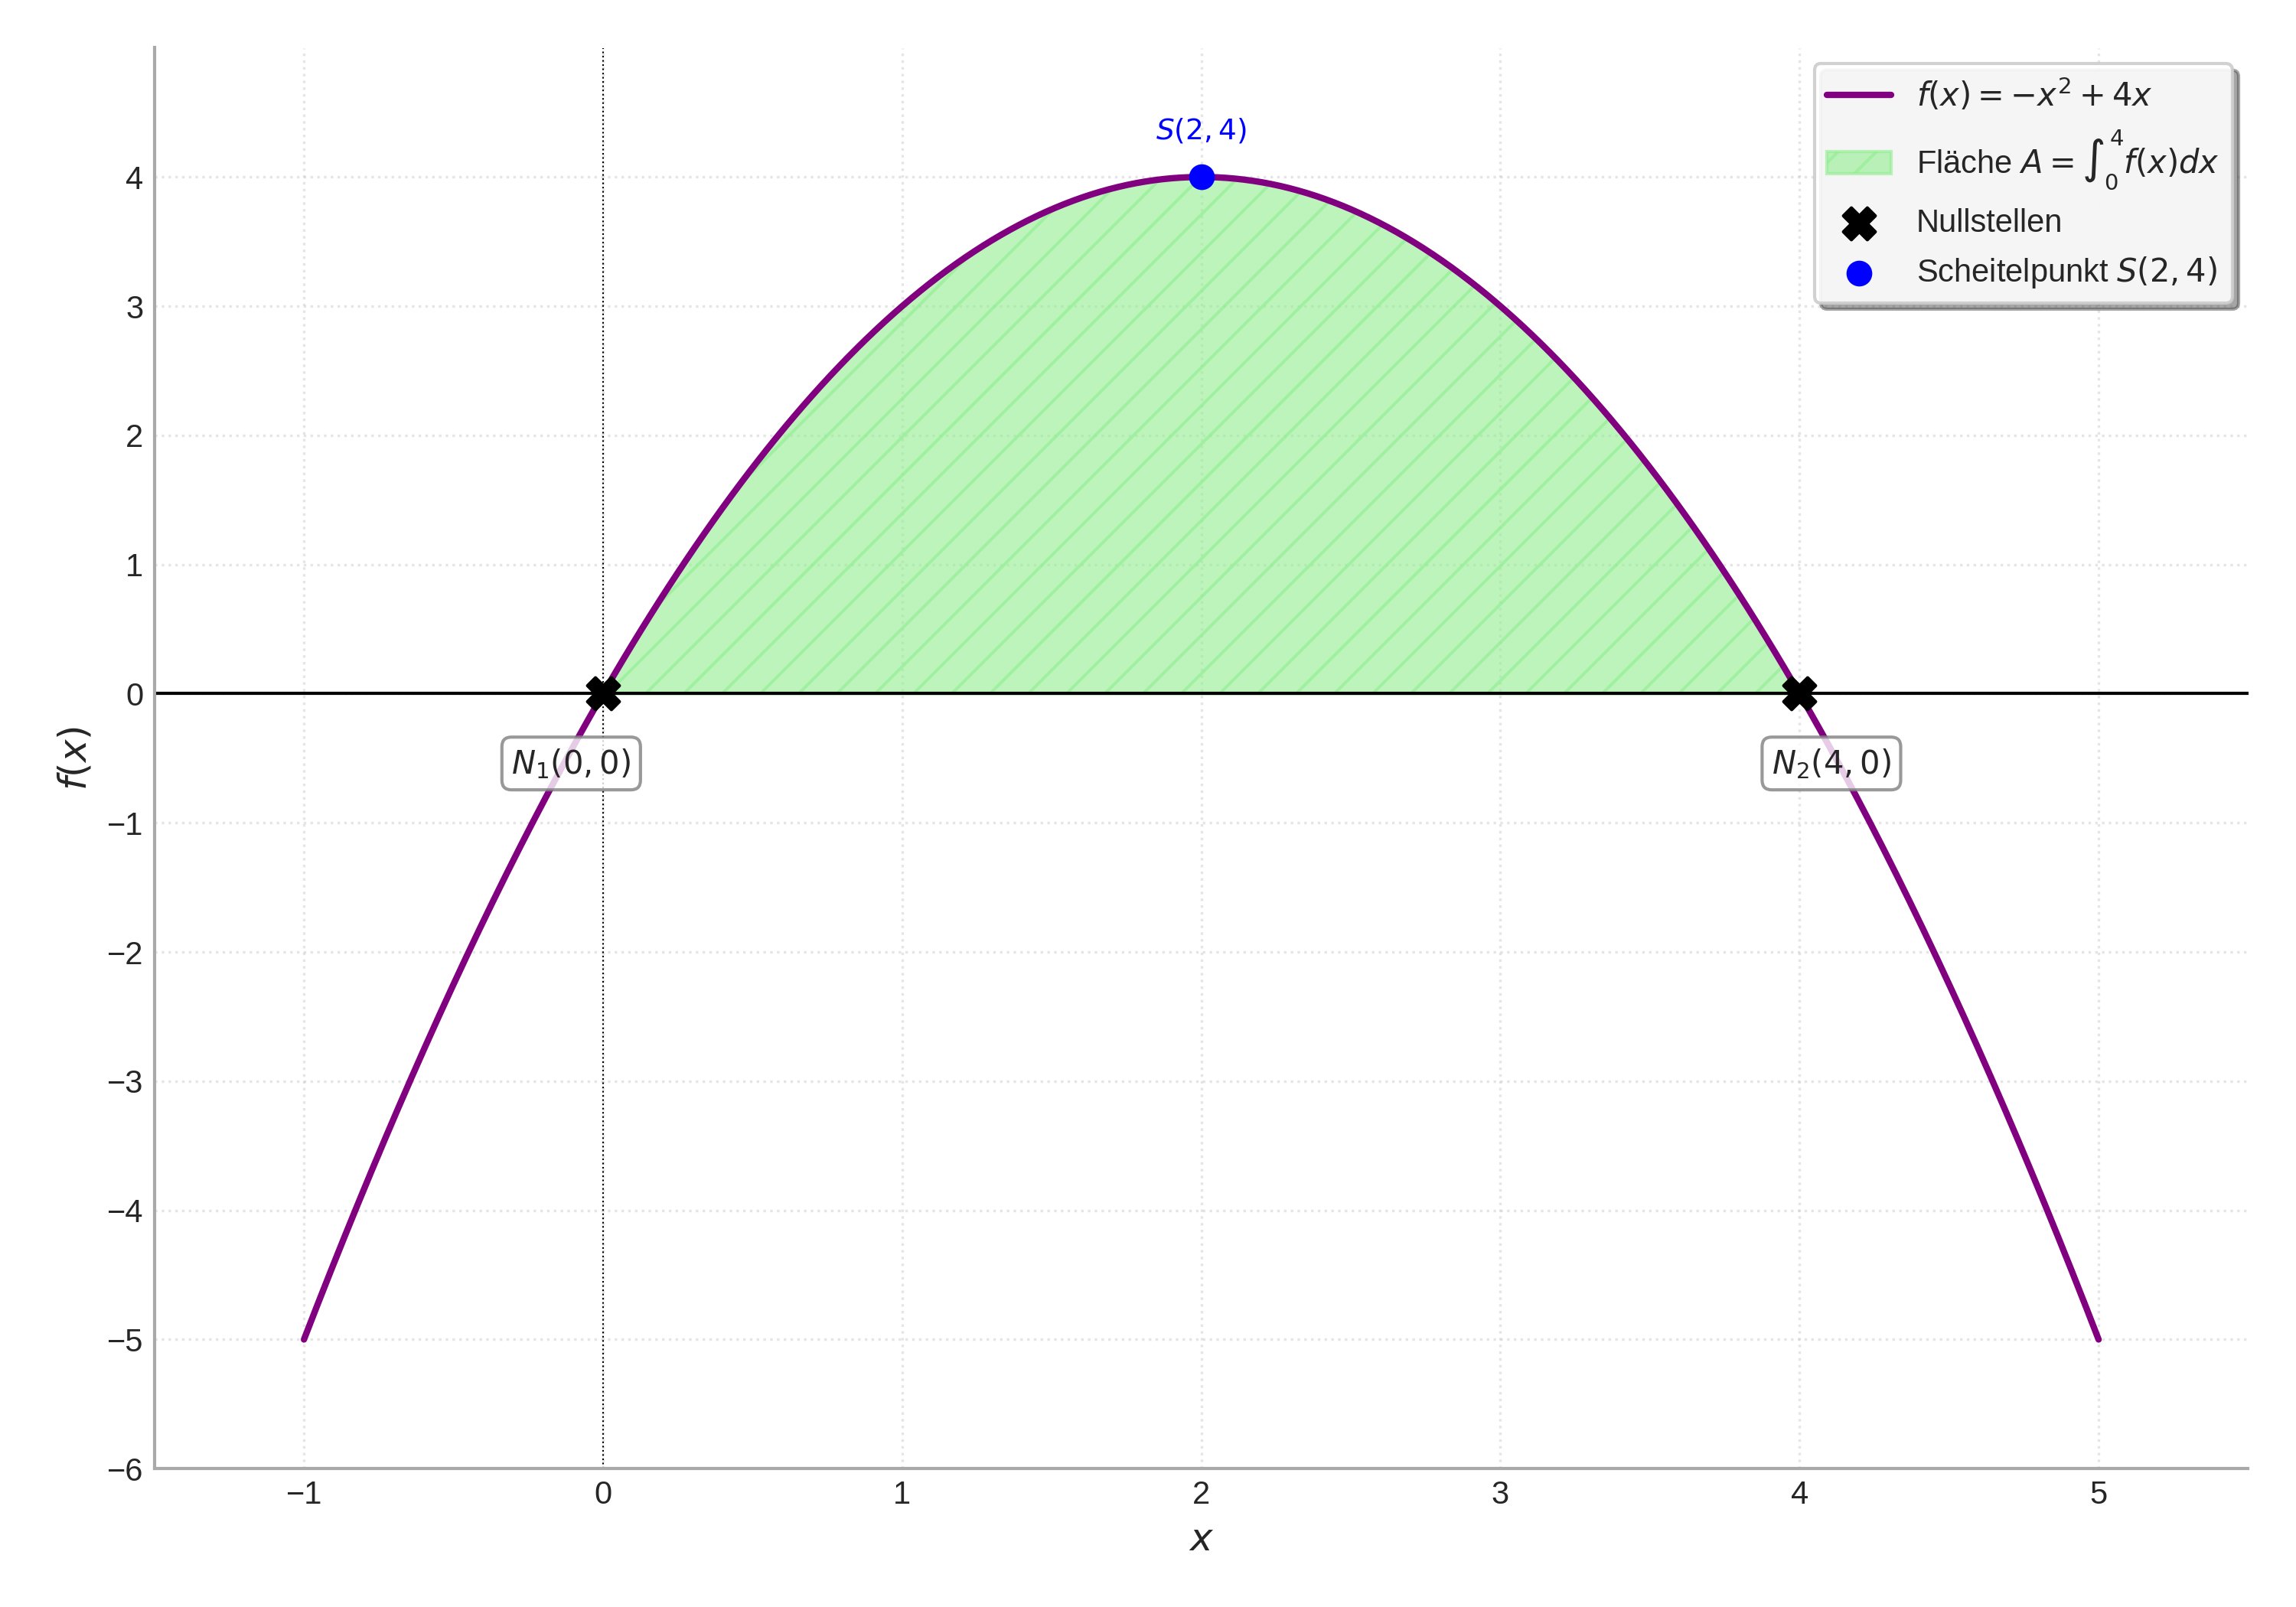
\includegraphics[width=0.8\textwidth]{grafiken/Integral_Flaeche_Parabel.png}
    \captionof{figure}{Fläche unter $f(x)=-x^2+4x$ zwischen den Nullstellen}
    \label{fig:flaeche_parabel}
\end{center}
        \end{itemize}
\end{enumerate}
\end{aufgabenumgebung}


\begin{funfactbox}{Newton, unendliche Reihen und die Quadratur des Kreises (fast!)}
Die Zahl $\pi$ fasziniert Mathematiker seit Jahrtausenden. Die alten Methoden zur Annäherung von $\pi$ waren oft geometrisch und extrem aufwendig. Isaac Newton fand um 1666 einen revolutionär neuen Weg, der die gerade erst entwickelte Analysis nutzte.

Seine Idee war, die Fläche eines Viertel-Einheitskreises zu berechnen, denn diese Fläche ist genau $\frac{\pi}{4}$. Die Gleichung eines Kreises mit Radius 1 ist $x^2+y^2=1$, also ist die obere Hälfte $y = \sqrt{1-x^2}$. Die Fläche des Viertelkreises im ersten Quadranten ist dann das bestimmte Integral:
\[ \text{Fläche} = \int_0^1 \sqrt{1-x^2} \,dx = \frac{\pi}{4} \]
Das Problem: Wie integriert man $\sqrt{1-x^2}$? Newton hatte dafür einen Trick! Er nutzte seine verallgemeinerte Form des \textbf{Binomialtheorems}, um $\sqrt{1-x^2}$ als eine \textbf{unendliche Summe (Reihe)} von Potenzen von $x$ darzustellen. Für $|x|<1$ lauten die ersten Terme dieser Reihe:
\[ \sqrt{1-x^2} = (1-x^2)^{\frac{1}{2}} = 1 - \frac{1}{2}x^2 - \frac{1}{8}x^4 - \frac{1}{16}x^6 - \frac{5}{128}x^8 - \dots \]
(Die genaue Herleitung dieser Koeffizienten ist etwas für Fortgeschrittene, aber die Idee ist, dass man den Ausdruck in eine 'unendlich langes Polynom' umwandelt.)

Das Geniale: Diese unendliche Summe konnte Newton nun Glied für Glied integrieren, ganz ähnlich wie du es bei Polynomen gelernt hast (Potenzregel der Integration: $\int x^n dx = \frac{1}{n+1}x^{n+1}$)!
\begin{align*} \int_0^1 \sqrt{1-x^2} \,dx &= \int_0^1 \left(1 - \frac{1}{2}x^2 - \frac{1}{8}x^4 - \frac{1}{16}x^6 - \dots \right) \,dx \\ &= \left[ x - \frac{1}{2 \cdot 3}x^3 - \frac{1}{8 \cdot 5}x^5 - \frac{1}{16 \cdot 7}x^7 - \dots \right]_0^1 \\ &= \left(1 - \frac{1}{6} - \frac{1}{40} - \frac{1}{112} - \dots \right) - (0) \end{align*}
Also erhielt Newton für $\pi/4$ die unendliche Reihe:
\[ \frac{\pi}{4} = 1 - \frac{1}{6} - \frac{1}{40} - \frac{1}{112} - \dots \]
Durch Aufsummieren von nur wenigen Termen dieser Reihe konnte Newton $\pi$ wesentlich genauer und schneller berechnen, als es mit den alten geometrischen Methoden möglich war. Er nutzte später sogar eine geschicktere Wahl der Integrationsgrenzen (von $0$ bis $1/2$), um eine Reihe zu erhalten, die noch schneller den Wert von $\pi$ liefert.

Dieser Ansatz zeigt eindrucksvoll, wie die Verbindung von unendlichen Reihen (oft aus der Differentialrechnung über Taylorreihen gewonnen) und der Integralrechnung völlig neue Wege zur Lösung alter Probleme eröffnete!

\begin{center}
    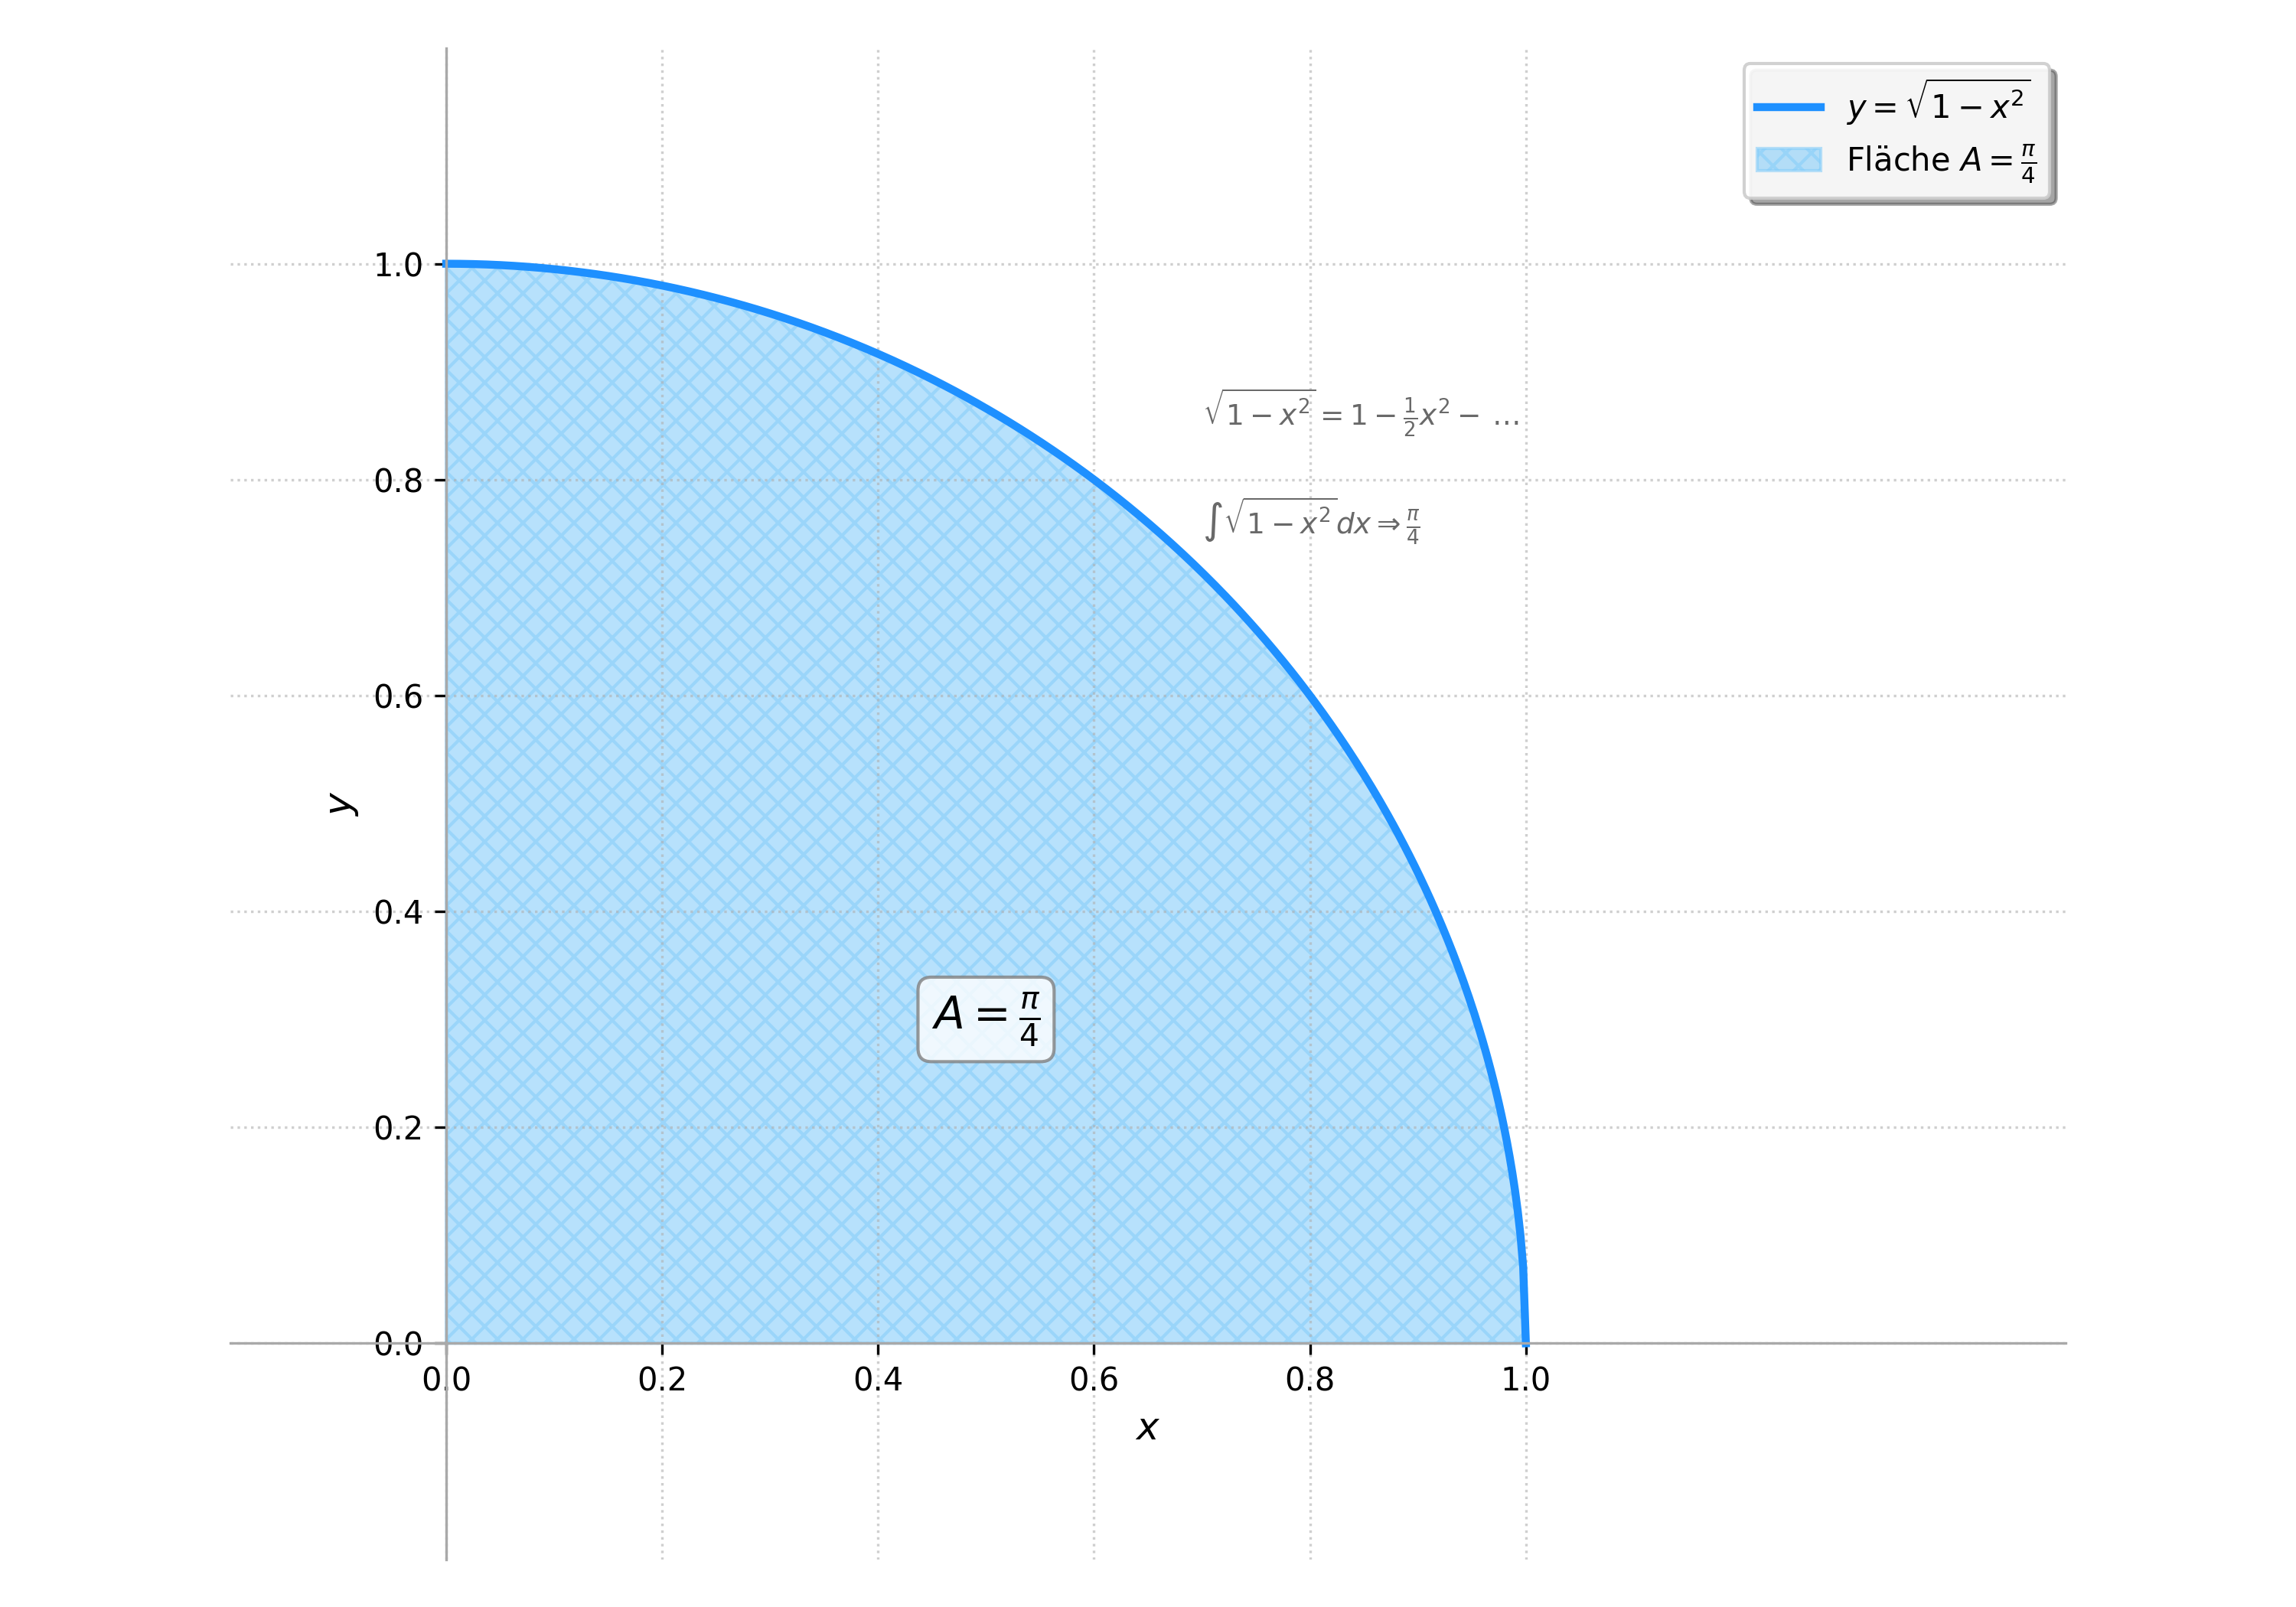
\includegraphics[width=0.6\textwidth]{grafiken/Newton_Pi_Integral.png}
    % Beschreibung für die Grafik 'Newton_Pi_Integral.png':
    % Die Grafik könnte den Graphen von y = sqrt(1-x^2) im ersten Quadranten zeigen (Viertelkreis).
    % Darunter die Fläche von x=0 bis x=1 schraffiert, beschriftet mit A = Pi/4.
    % Daneben oder darunter die ersten Terme der Reihe für sqrt(1-x^2) und 
    % die ersten Terme der integrierten Reihe für Pi/4.
    % Optional ein kleines Portrait von Newton.
    \captionof{figure}{Konzept der $\pi$-Berechnung durch Integration der Binomialreihe für den Viertelkreis}
    \label{fig:newton_pi_integral_funfact}
\end{center}
\end{funfactbox}

\subsubsection{Anwendungen und Interpretationen des bestimmten Integrals}

Die wichtigste geometrische Interpretation des bestimmten Integrals $\int_a^b f(x)dx$ ist, wie erwähnt, der orientierte Flächeninhalt zwischen dem Graphen von $f(x)$ und der x-Achse im Intervall $[a,b]$.

\begin{infoboxumgebung}{Flächenberechnung bei Nullstellen und unterhalb der x-Achse}
Wenn eine Funktion $f(x)$ im Integrationsintervall $[a,b]$ Nullstellen besitzt und somit Teile des Graphen unterhalb der x-Achse liegen, liefert das bestimmte Integral $\int_a^b f(x)dx$ die \textbf{Flächenbilanz}. Das bedeutet, Flächenstücke oberhalb der x-Achse werden positiv gewertet, Flächenstücke unterhalb der x-Achse negativ.

Um den \textbf{tatsächlichen geometrischen Flächeninhalt} zu berechnen, der zwischen dem Graphen und der x-Achse eingeschlossen wird, musst du:
\begin{enumerate}
    \item Die Nullstellen $x_N$ der Funktion im Intervall $[a,b]$ finden.
    \item Das Integral über die Teilintervalle berechnen, die durch die Nullstellen entstehen.
    \item Die \textbf{Beträge} der Integralteile addieren, bei denen der Graph unterhalb der x-Achse verläuft (also wo das Integral negativ wäre).
\end{enumerate}
Mathematisch entspricht das der Berechnung von $\int_a^b |f(x)| \,dx$. In der Praxis ist es oft einfacher, die Teilintegrale zu berechnen und dann die Beträge zu addieren.

Beispiel: Wenn $f(x)$ eine Nullstelle $x_N$ zwischen $a$ und $b$ hat und $f(x) \ge 0$ für $x \in [a, x_N]$ und $f(x) \le 0$ für $x \in [x_N, b]$, dann ist der Gesamtflächeninhalt $A_{ges}$:
\[ A_{ges} = \int_a^{x_N} f(x) \,dx + \left| \int_{x_N}^b f(x) \,dx \right| = \int_a^{x_N} f(x) \,dx - \int_{x_N}^b f(x) \,dx \]
(Da $\int_{x_N}^b f(x) \,dx$ negativ wäre, wird durch das Minuszeichen der Betrag addiert).
\end{infoboxumgebung}

\begin{beispielumgebung}{Fläche mit Anteilen unter der x-Achse}
Berechne den Flächeninhalt, den der Graph der Funktion $f(x) = x^2 - 1$ mit der x-Achse im Intervall $[-2, 2]$ einschließt.

\textbf{Schritt 1: Nullstellen von $f(x)$ finden.}
$x^2 - 1 = 0 \implies x^2 = 1 \implies x_{N1} = -1, x_{N2} = 1$.
Beide Nullstellen liegen im Intervall $[-2,2]$.

\textbf{Schritt 2: Vorzeichen von $f(x)$ in den Teilintervallen bestimmen.}
Die Parabel $f(x)=x^2-1$ ist nach oben geöffnet.
\begin{itemize}
    \item Intervall $[-2, -1]$: z.B. $f(-1.5) = (-1.5)^2-1 = 2.25-1 = 1.25 > 0$. (Graph oberhalb)
    \item Intervall $[-1, 1]$: z.B. $f(0) = 0^2-1 = -1 < 0$. (Graph unterhalb)
    \item Intervall $[1, 2]$: z.B. $f(1.5) = (1.5)^2-1 = 2.25-1 = 1.25 > 0$. (Graph oberhalb)
\end{itemize}

\textbf{Schritt 3: Teilintegrale berechnen.}
Stammfunktion $F(x) = \frac{1}{3}x^3 - x$.
$A_1 = \int_{-2}^{-1} (x^2-1) \,dx = [\frac{1}{3}x^3-x]_{-2}^{-1} = (\frac{1}{3}(-1)^3 - (-1)) - (\frac{1}{3}(-2)^3 - (-2))$
$= (-\frac{1}{3}+1) - (-\frac{8}{3}+2) = \frac{2}{3} - (-\frac{8}{3}+\frac{6}{3}) = \frac{2}{3} - (-\frac{2}{3}) = \frac{2}{3} + \frac{2}{3} = \frac{4}{3}$.

$A_2 = \int_{-1}^{1} (x^2-1) \,dx = [\frac{1}{3}x^3-x]_{-1}^{1} = (\frac{1}{3}(1)^3 - 1) - (\frac{1}{3}(-1)^3 - (-1))$
$= (\frac{1}{3}-1) - (-\frac{1}{3}+1) = -\frac{2}{3} - \frac{2}{3} = -\frac{4}{3}$.
(Das Integral ist negativ, da die Fläche unter der x-Achse liegt. Der Flächen\textit{inhalt} ist $|-\frac{4}{3}| = \frac{4}{3}$).

$A_3 = \int_{1}^{2} (x^2-1) \,dx = [\frac{1}{3}x^3-x]_{1}^{2} = (\frac{1}{3}(2)^3 - 2) - (\frac{1}{3}(1)^3 - 1)$
$= (\frac{8}{3}-2) - (\frac{1}{3}-1) = (\frac{8}{3}-\frac{6}{3}) - (-\frac{2}{3}) = \frac{2}{3} + \frac{2}{3} = \frac{4}{3}$.

\textbf{Schritt 4: Gesamtflächeninhalt.}
$A_{ges} = A_1 + |A_2| + A_3 = \frac{4}{3} + \frac{4}{3} + \frac{4}{3} = \frac{12}{3} = 4$.
Der Gesamtflächeninhalt beträgt 4 Flächeneinheiten.
\begin{center}
    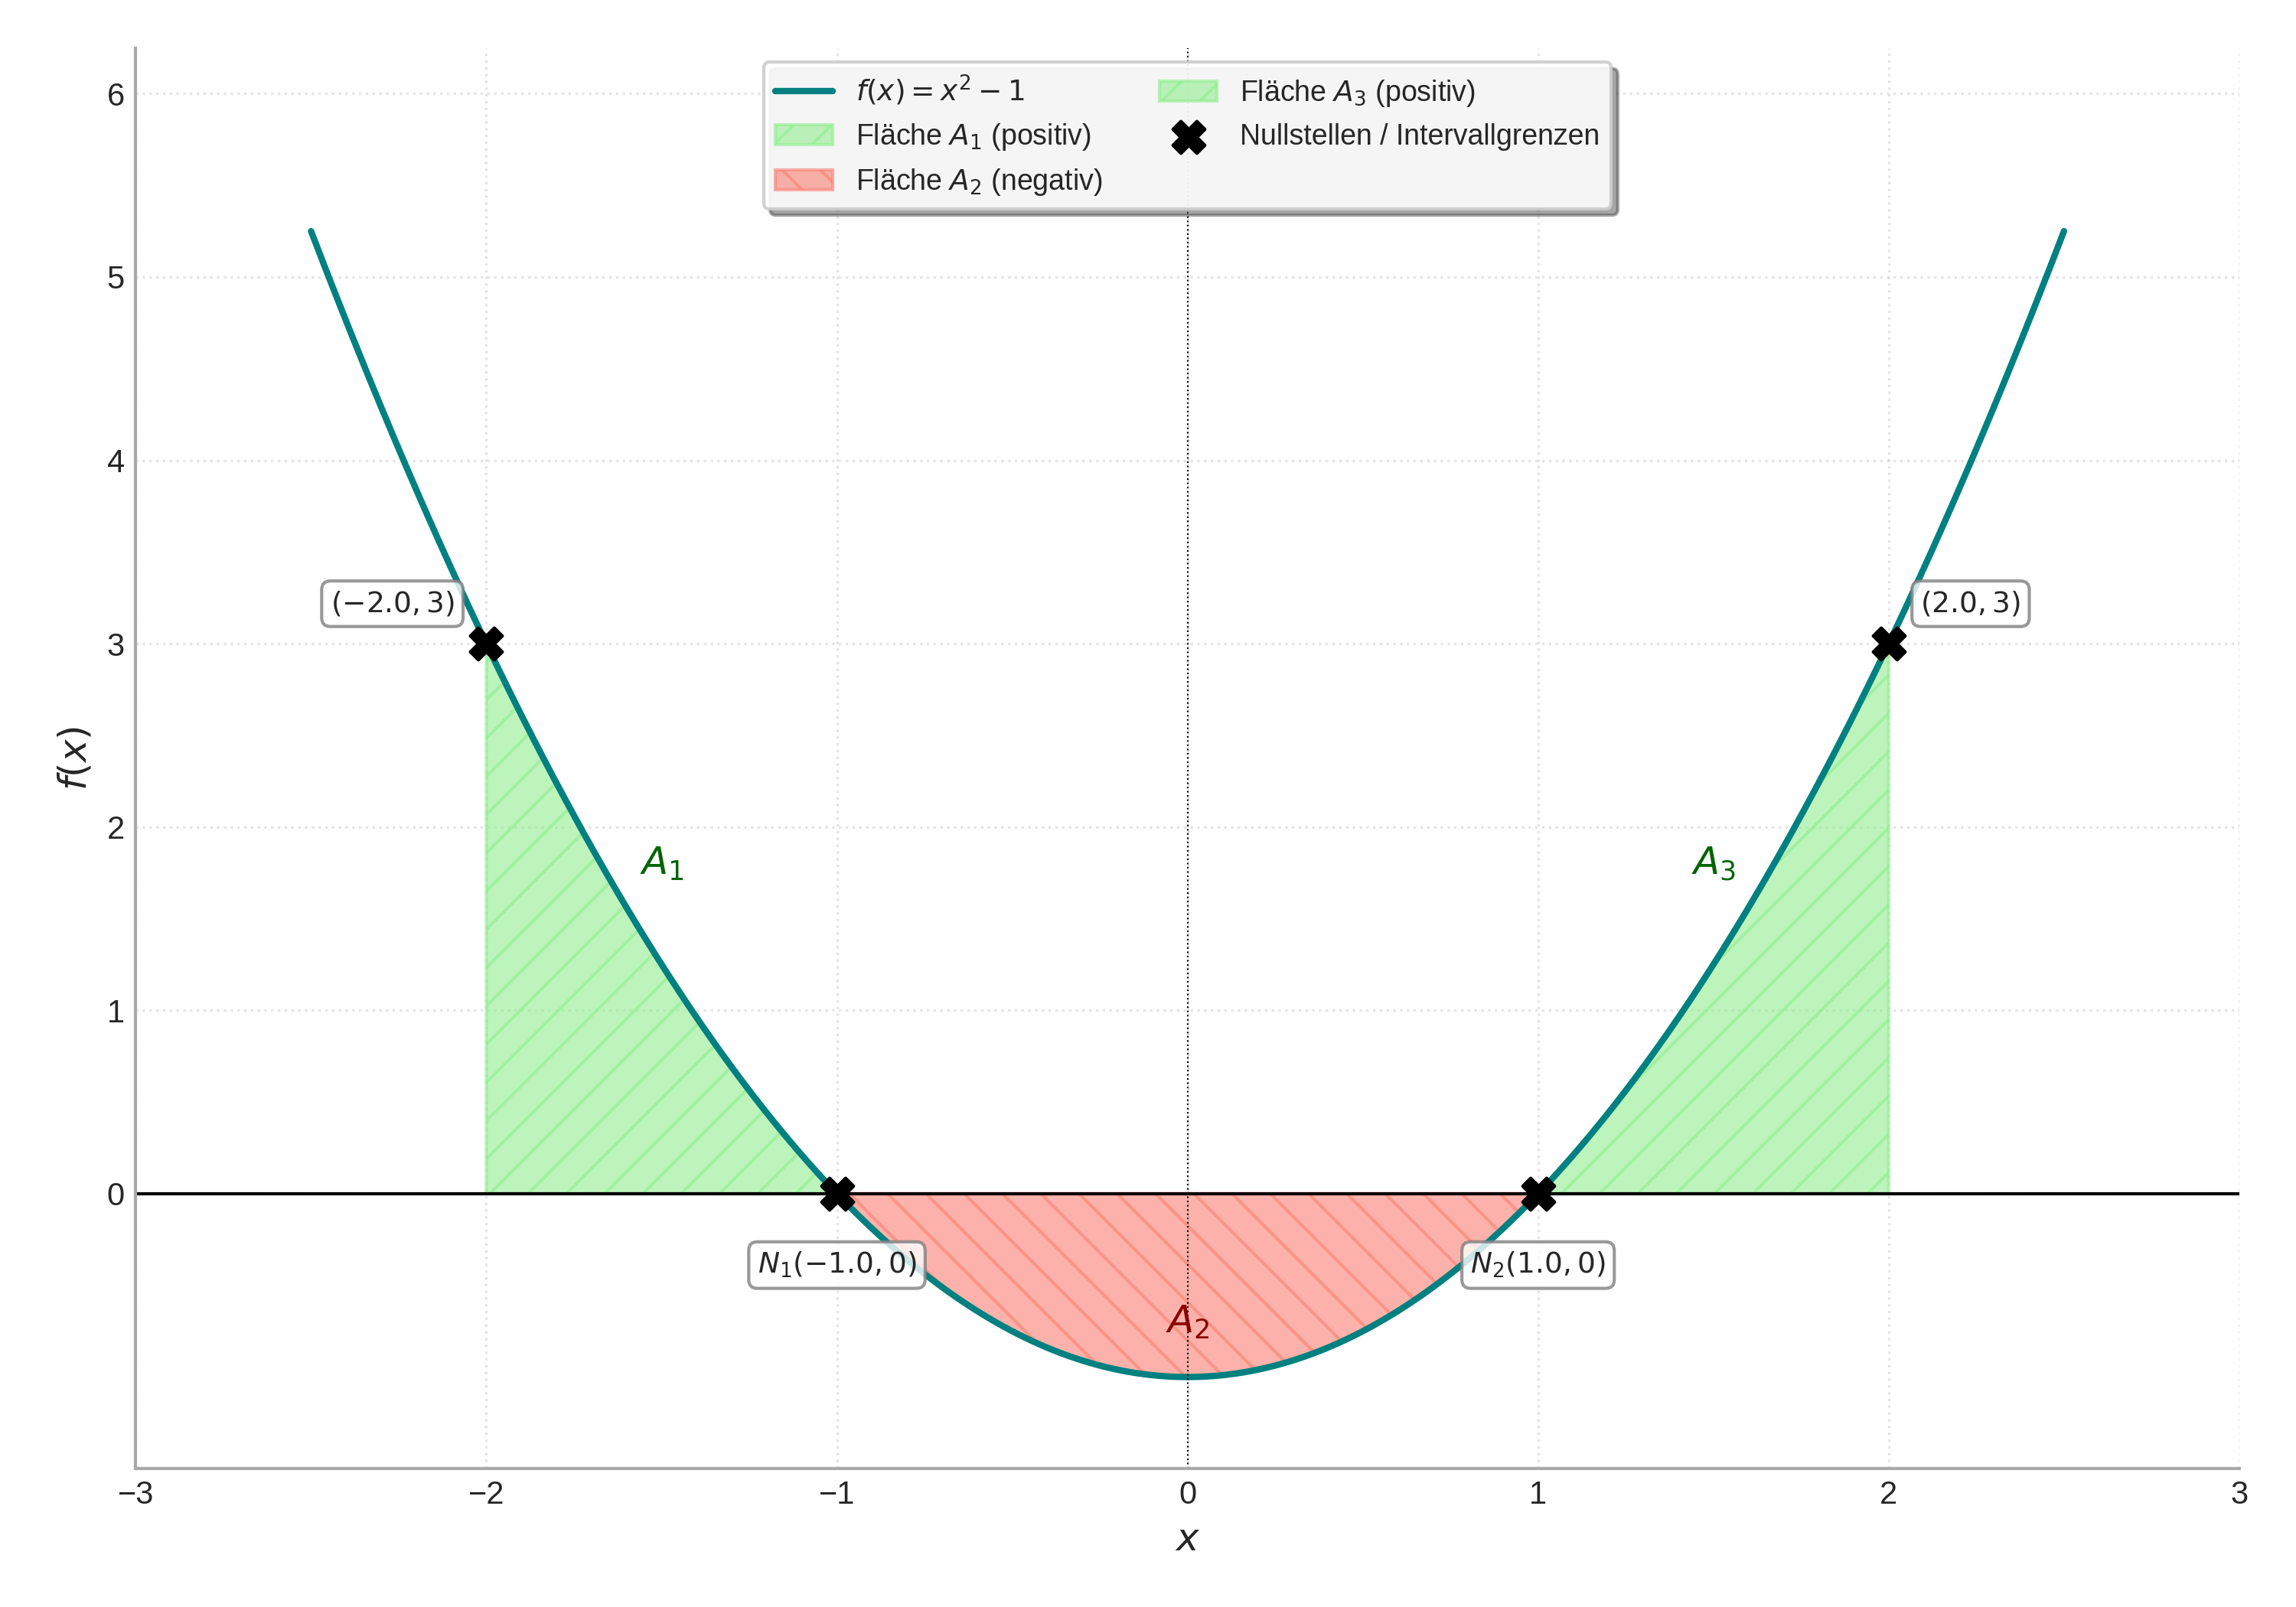
\includegraphics[width=0.8\textwidth]{grafiken/Integral_Flaeche_xhoch2minus1.png}
    \captionof{figure}{Fläche zwischen $f(x)=x^2-1$ und der x-Achse von -2 bis 2}
    \label{fig:flaeche_x2minus1}
\end{center}
\end{beispielumgebung}

\begin{aufgabenumgebung}{Flächenberechnung mit Nullstellen im Intervall}
Berechne den Inhalt der Fläche, die vom Graphen der Funktion $f(x) = x^3 - x$ und der x-Achse im Intervall $[-2, 2]$ eingeschlossen wird.
\begin{tippumgebung}{Vorgehen}
\begin{enumerate}
    \item Skizziere den Graphen (oder überlege dir den Verlauf anhand von Symmetrie und Nullstellen).
    \item Finde alle Nullstellen von $f(x)$.
    \item Bestimme, in welchen Teilintervallen $f(x) \ge 0$ und in welchen $f(x) \le 0$ ist.
    \item Berechne die bestimmten Integrale über die Teilintervalle und addiere deren Beträge.
\end{enumerate}
\end{tippumgebung}
\end{aufgabenumgebung}

\begin{infoboxumgebung}{Symmetrie und bestimmte Integrale – Rechnungen vereinfachen!}
Die Symmetrieeigenschaften von Funktionen können uns die Berechnung bestimmter Integrale oft erheblich erleichtern, besonders wenn das Integrationsintervall symmetrisch zum Ursprung ist (also von der Form $[-a, a]$).

\begin{itemize}
    \item \textbf{Punktsymmetrie zum Ursprung:}
        Wenn eine Funktion $f(x)$ punktsymmetrisch zum Ursprung ist (d.h. $f(-x) = -f(x)$, wie z.B. bei $x, x^3, x^5, \sin(x)$), dann gilt für jedes $a>0$:
        \[ \int_{-a}^{a} f(x) \,dx = 0 \]
        \textit{Warum?} Die Fläche links vom Ursprung (unterhalb der x-Achse, wenn $f(x)$ für $x>0$ oberhalb ist) ist genauso groß wie die Fläche rechts vom Ursprung (oberhalb der x-Achse), aber mit entgegengesetztem Vorzeichen. Sie heben sich also gegenseitig auf.
        \begin{center}
            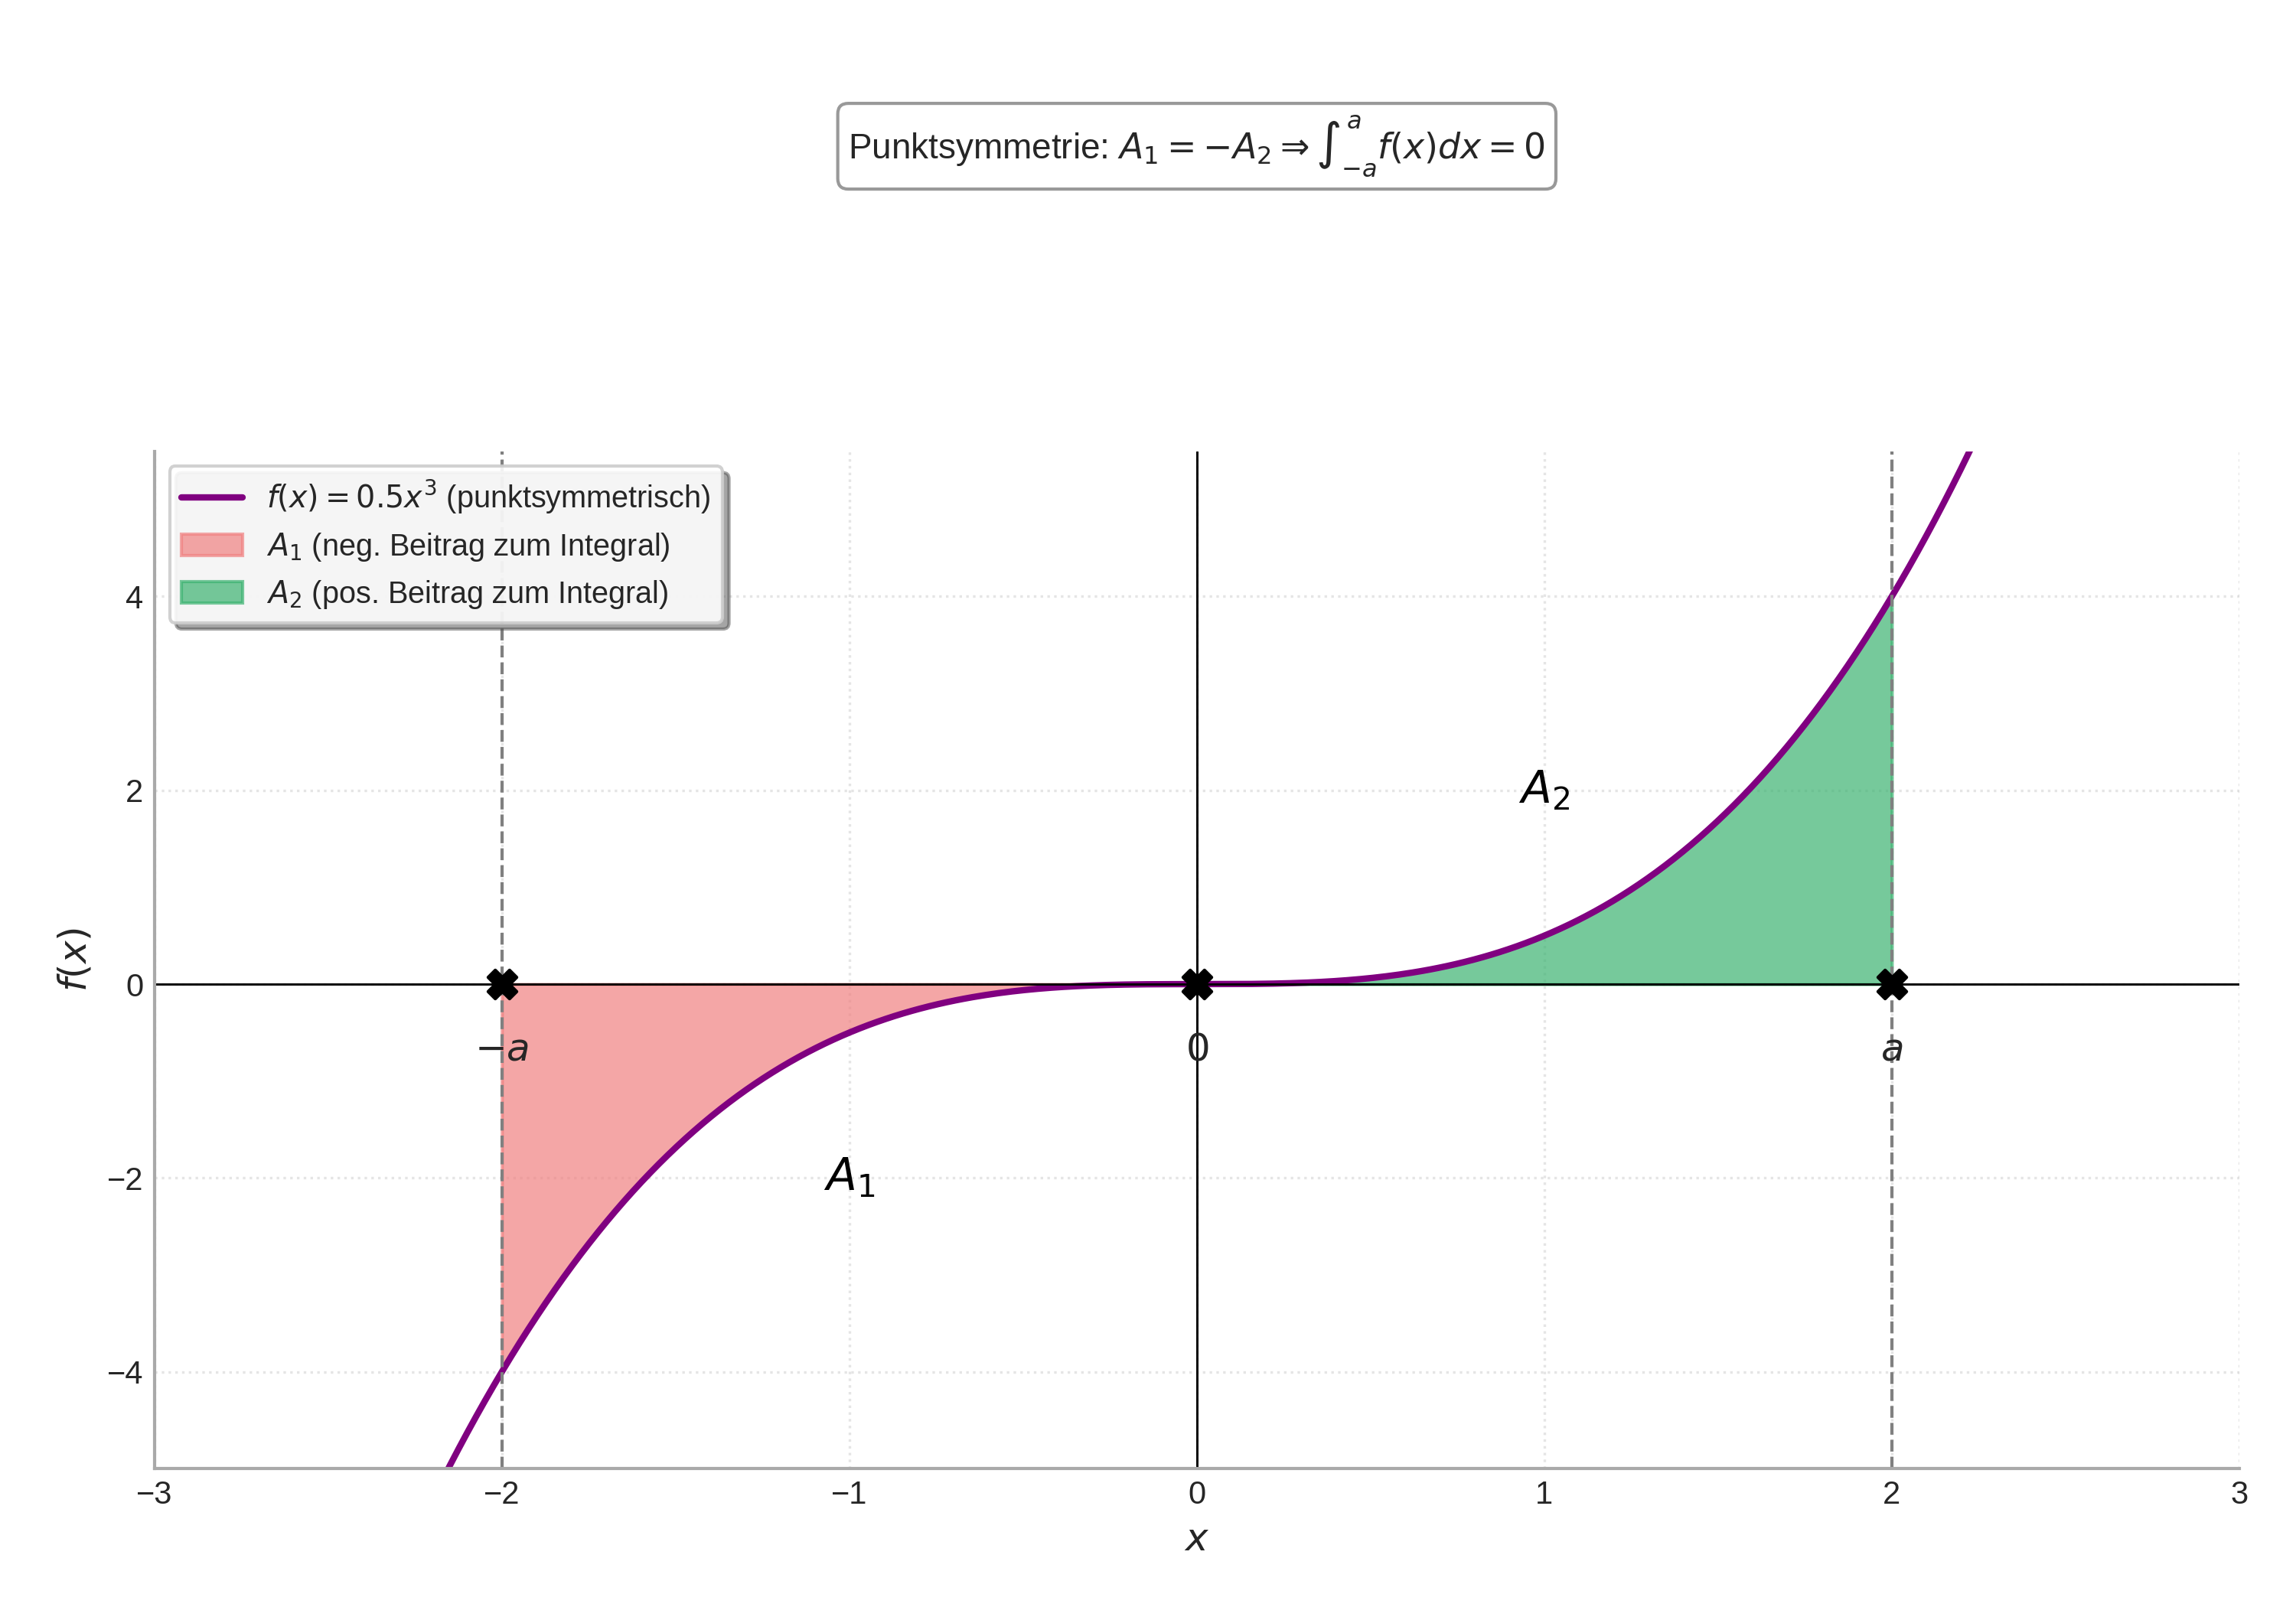
\includegraphics[width=0.7\textwidth]{grafiken/Integral_Punktsymmetrie.png}
            \captionof{figure}{Integral einer punktsymmetrischen Funktion über $[-a,a]$}
            \label{fig:integral_punktsymmetrie}
        \end{center}

    \item \textbf{Achsensymmetrie zur y-Achse:}
        Wenn eine Funktion $f(x)$ achsensymmetrisch zur y-Achse ist (d.h. $f(-x) = f(x)$, wie z.B. bei $x^2, x^4, |x|, \cos(x)$), dann gilt für jedes $a>0$:
        \[ \int_{-a}^{a} f(x) \,dx = 2 \cdot \int_{0}^{a} f(x) \,dx \]
        \textit{Warum?} Die Fläche links von der y-Achse (von $-a$ bis $0$) ist genauso groß wie die Fläche rechts von der y-Achse (von $0$ bis $a$). Man kann also die Rechnung vereinfachen, indem man nur eine Hälfte berechnet und das Ergebnis verdoppelt.
        % \begin{center}
        %     % Platzhalter für die Grafik 'Integral Achsensymmetrie'
        %     \framebox{\begin{minipage}{0.7\textwidth}
        %         \centering \vspace{1.5cm}
        %         \textbf{Platzhalter: Integral\_Achsensymmetrie.png} \\
        %         Beschreibung: Graph einer achsensymmetrischen Funktion (z.B. $x^2$) über $[-a,a]$. Die Fläche $A_1$ von $-a$ bis $0$ und $A_2$ von $0$ bis $a$ sind gleich groß und haben das gleiche Vorzeichen.
        %         \vspace{1.5cm}
        %     \end{minipage}}
        %     \captionof{figure}{Integral einer achsensymmetrischen Funktion über $[-a,a]$ (Platzhalter).}
        % \end{center}
        \begin{center}
            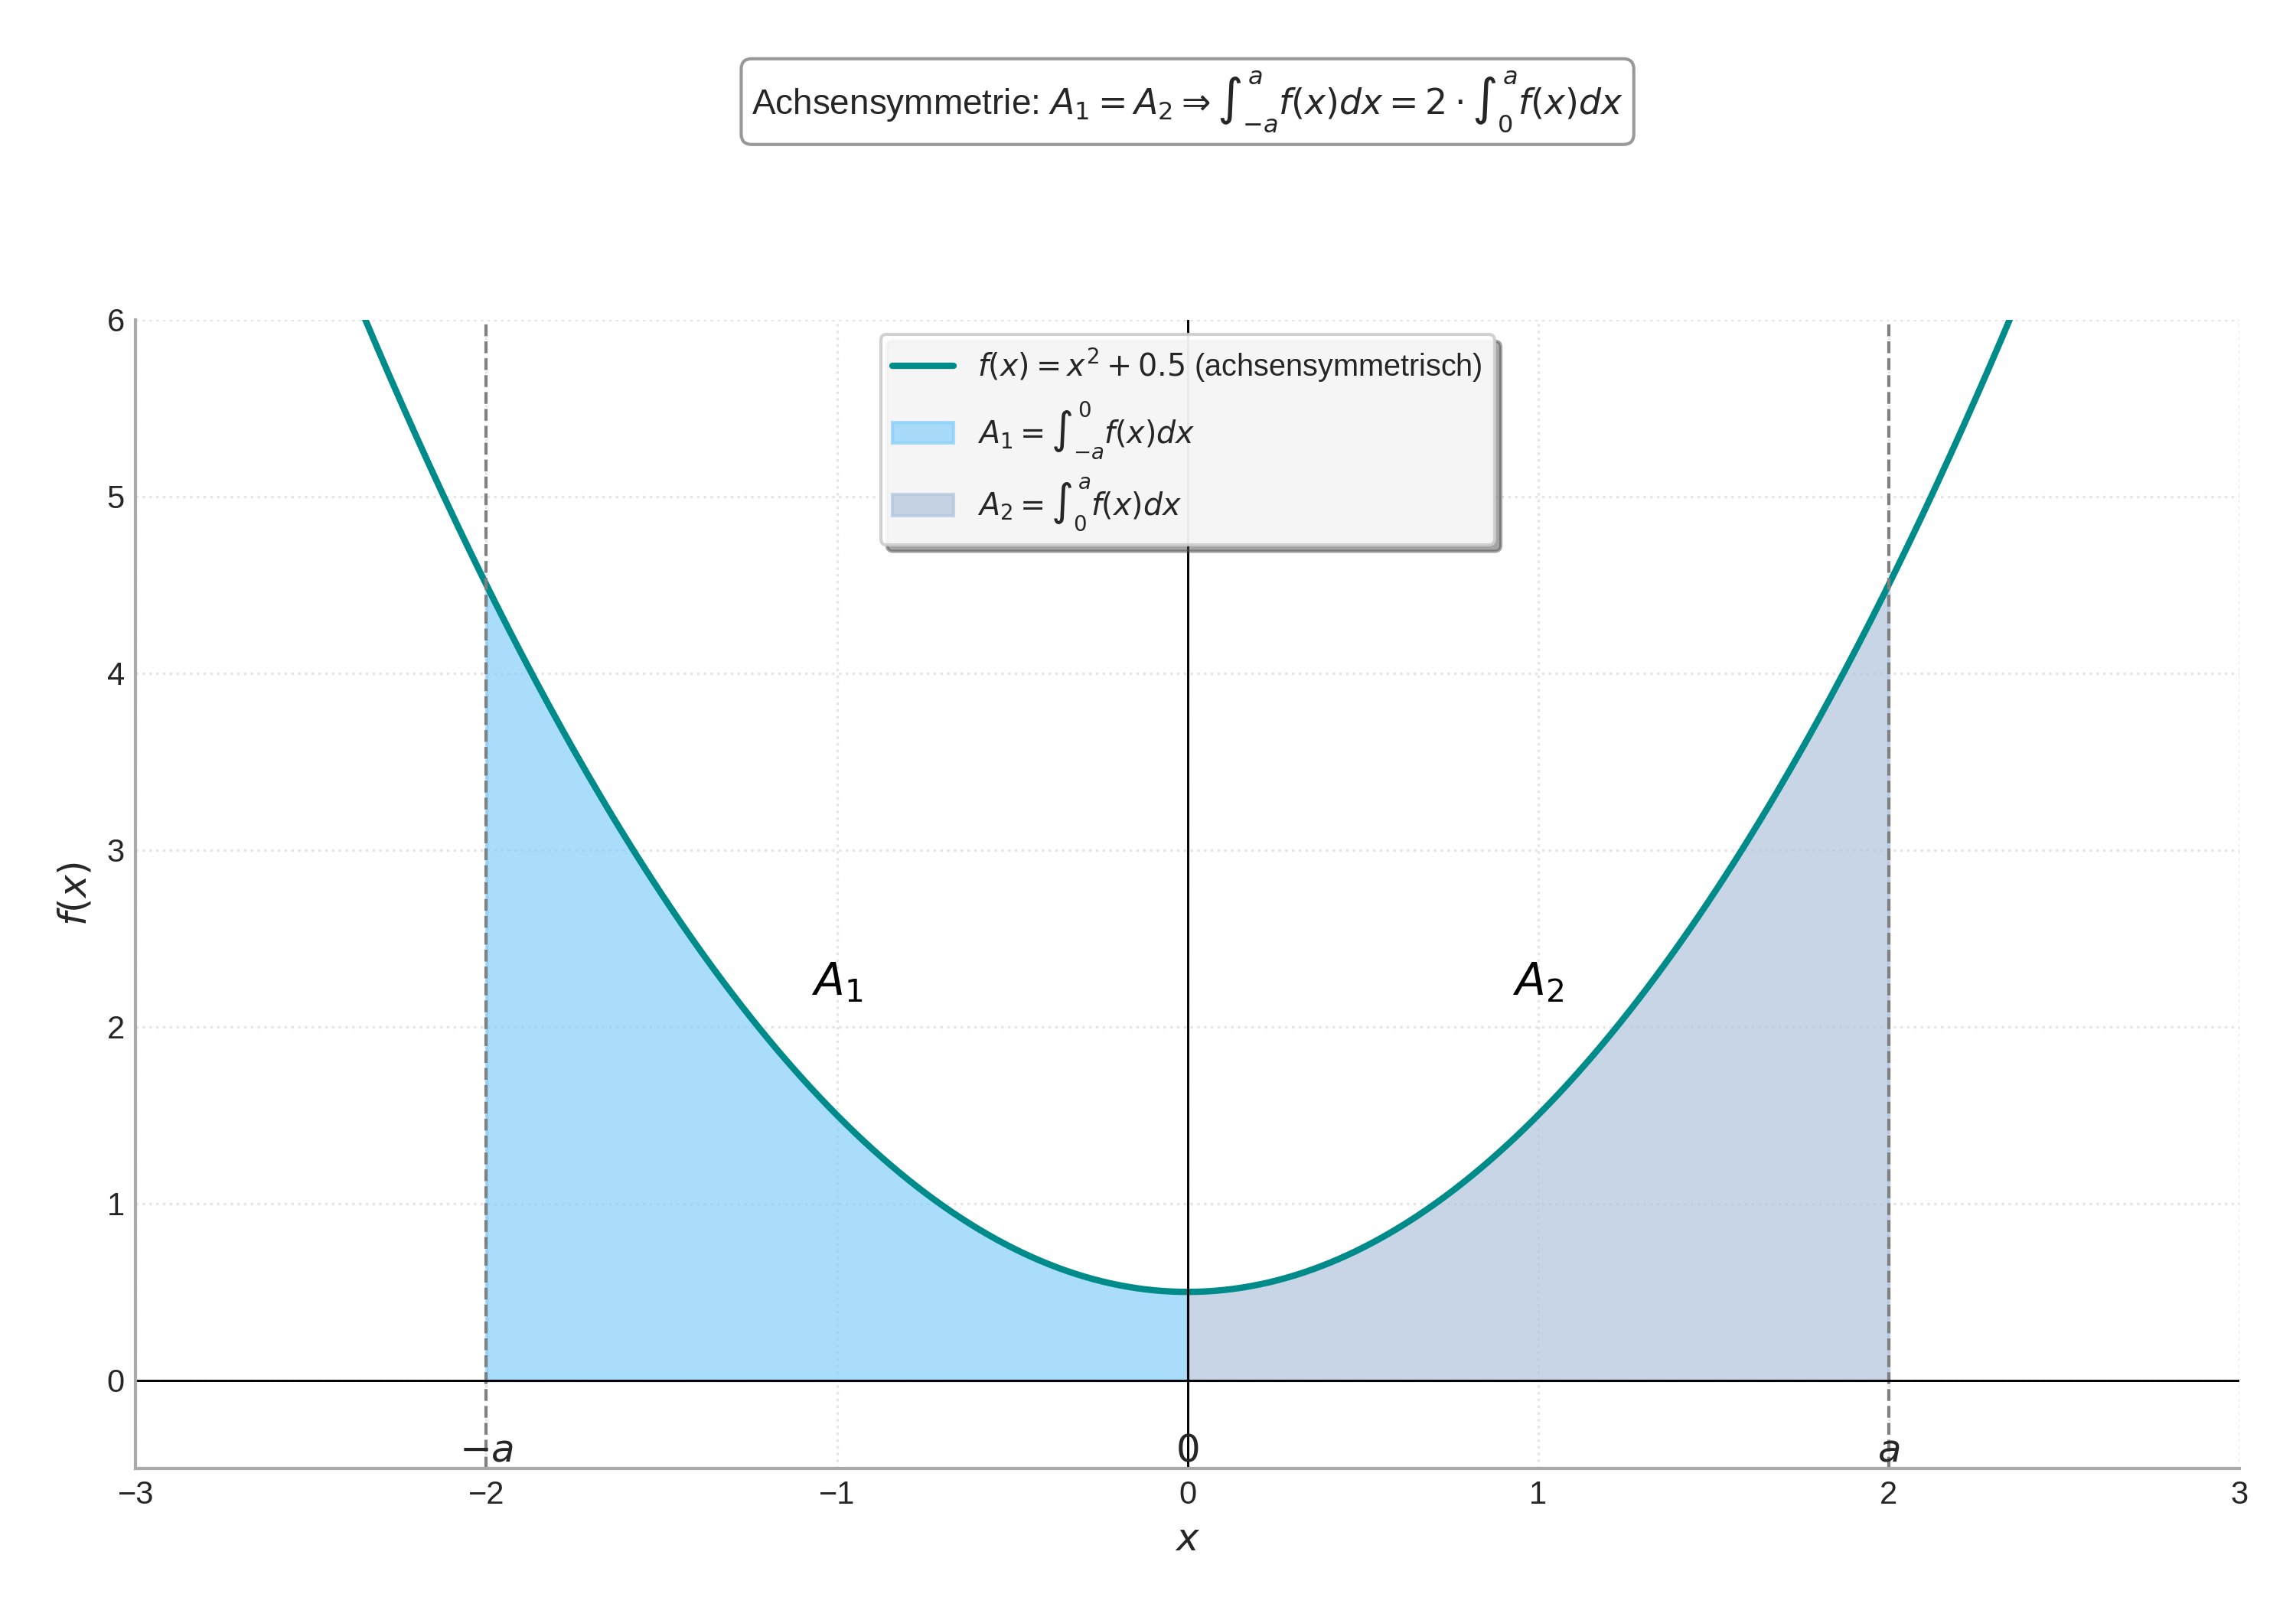
\includegraphics[width=0.7\textwidth]{grafiken/Integral_Achsensymmetrie.png}
            \captionof{figure}{Integral einer achsensymmetrischen Funktion über $[-a,a]$}
            \label{fig:integral_achsensymmetrie}
        \end{center}
\end{itemize}
Diese Symmetrieüberlegungen können dir viel Rechenarbeit ersparen!
\end{infoboxumgebung}

\begin{beispielumgebung}{Symmetrie beim Integrieren nutzen}
\begin{enumerate}
    \item Berechne $\int_{-1}^{1} x^3 \,dx$.
        Die Funktion $f(x)=x^3$ ist punktsymmetrisch zum Ursprung, da $f(-x)=(-x)^3 = -x^3 = -f(x)$.
        Das Integrationsintervall $[-1,1]$ ist symmetrisch zum Ursprung.
        Daher gilt: $\int_{-1}^{1} x^3 \,dx = 0$.
        \textit{Probe (mit HDI):} $F(x) = \frac{1}{4}x^4$.
        $[ \frac{1}{4}x^4 ]_{-1}^{1} = (\frac{1}{4}(1)^4) - (\frac{1}{4}(-1)^4) = \frac{1}{4} - \frac{1}{4} = 0$. Stimmt!

    \item Berechne $\int_{-2}^{2} (3x^2 - 5) \,dx$.
        Die Funktion $f(x)=3x^2-5$ ist achsensymmetrisch zur y-Achse, da sie nur gerade Potenzen von $x$ enthält (und eine Konstante): $f(-x) = 3(-x)^2-5 = 3x^2-5 = f(x)$.
        Das Intervall $[-2,2]$ ist symmetrisch.
        Daher: $\int_{-2}^{2} (3x^2 - 5) \,dx = 2 \cdot \int_{0}^{2} (3x^2 - 5) \,dx$.
        Stammfunktion $F(x) = x^3 - 5x$.
        $2 \cdot [x^3 - 5x]_{0}^{2} = 2 \cdot ( ( (2)^3 - 5(2) ) - ( (0)^3 - 5(0) ) )$
        $= 2 \cdot ( (8 - 10) - (0) ) = 2 \cdot (-2) = -4$.
\end{enumerate}
\end{beispielumgebung}

\begin{aufgabenumgebung}{Symmetrie beim Integrieren anwenden}
Berechne die folgenden bestimmten Integrale. Nutze Symmetrieeigenschaften, wenn möglich, um die Rechnung zu vereinfachen.
\begin{enumerate}
    \item $\int_{-5}^{5} (x^5 - 2x^3 + x) \,dx$
    \item $\int_{-1}^{1} (x^4 + 3x^2 - 1) \,dx$
    \item $\int_{-\pi}^{\pi} \sin(x) \,dx$ (Du weißt vielleicht schon, dass $\sin(x)$ punktsymmetrisch ist. Die Stammfunktion von $\sin(x)$ ist $-\cos(x)$.)
\end{enumerate}
\end{aufgabenumgebung}

% Hier geht es dann weiter mit weiteren Anwendungen oder dem Abschluss des Kapitels.

% Vorheriger Inhalt des Kapitels bis zur aufgabenumgebung 'Symmetrie beim Integrieren anwenden'
% ... (siehe vorherige Canvas-Version) ...

\begin{aufgabenumgebung}{Fläche zwischen zwei Kurven}
Die Graphen der Funktionen $f(x) = -x^2 + 4x + 1$ und $g(x) = x^2 - 2x + 1$ schließen eine Fläche ein.
\begin{enumerate}
    \item \textbf{Schnittpunkte bestimmen:} Berechne die x-Koordinaten der Schnittpunkte der beiden Graphen, indem du $f(x) = g(x)$ setzt und die entstehende Gleichung löst. Diese Schnittpunkte sind deine Integrationsgrenzen $a$ und $b$.
    \item \textbf{Welche Funktion liegt oben?} Bestimme, welche der beiden Funktionen im Intervall $[a,b]$ die größeren Funktionswerte hat (also 'oben' liegt). Du kannst dies tun, indem du einen Testwert aus dem Intervall $(a,b)$ in beide Funktionen einsetzt oder die Graphen skizzierst.
    \item \textbf{Differenzfunktion bilden:} Bilde die Differenzfunktion $d(x) = \text{obere Funktion} - \text{untere Funktion}$.
    \item \textbf{Flächeninhalt berechnen:} Berechne den Flächeninhalt $A = \int_a^b d(x) \,dx$.
    \item \textbf{Skizze:} Skizziere beide Parabeln und die eingeschlossene Fläche in ein Koordinatensystem.
\end{enumerate}
\begin{merksatzumgebung}{Fläche zwischen zwei Graphen}
Den Flächeninhalt $A$ zwischen den Graphen zweier Funktionen $f(x)$ und $g(x)$ im Intervall $[a,b]$, wobei $f(x) \ge g(x)$ für alle $x \in [a,b]$ gilt (d.h. $f(x)$ ist die obere Funktion), berechnet man mit:
\[ A = \int_a^b (f(x) - g(x)) \,dx \]
Wenn nicht klar ist, welche Funktion oben liegt, oder wenn sich die obere Funktion ändert, muss man das Intervall entsprechend aufteilen und/oder den Betrag der Differenz integrieren: $A = \int_a^b |f(x) - g(x)| \,dx$.
\end{merksatzumgebung}
\begin{center}
    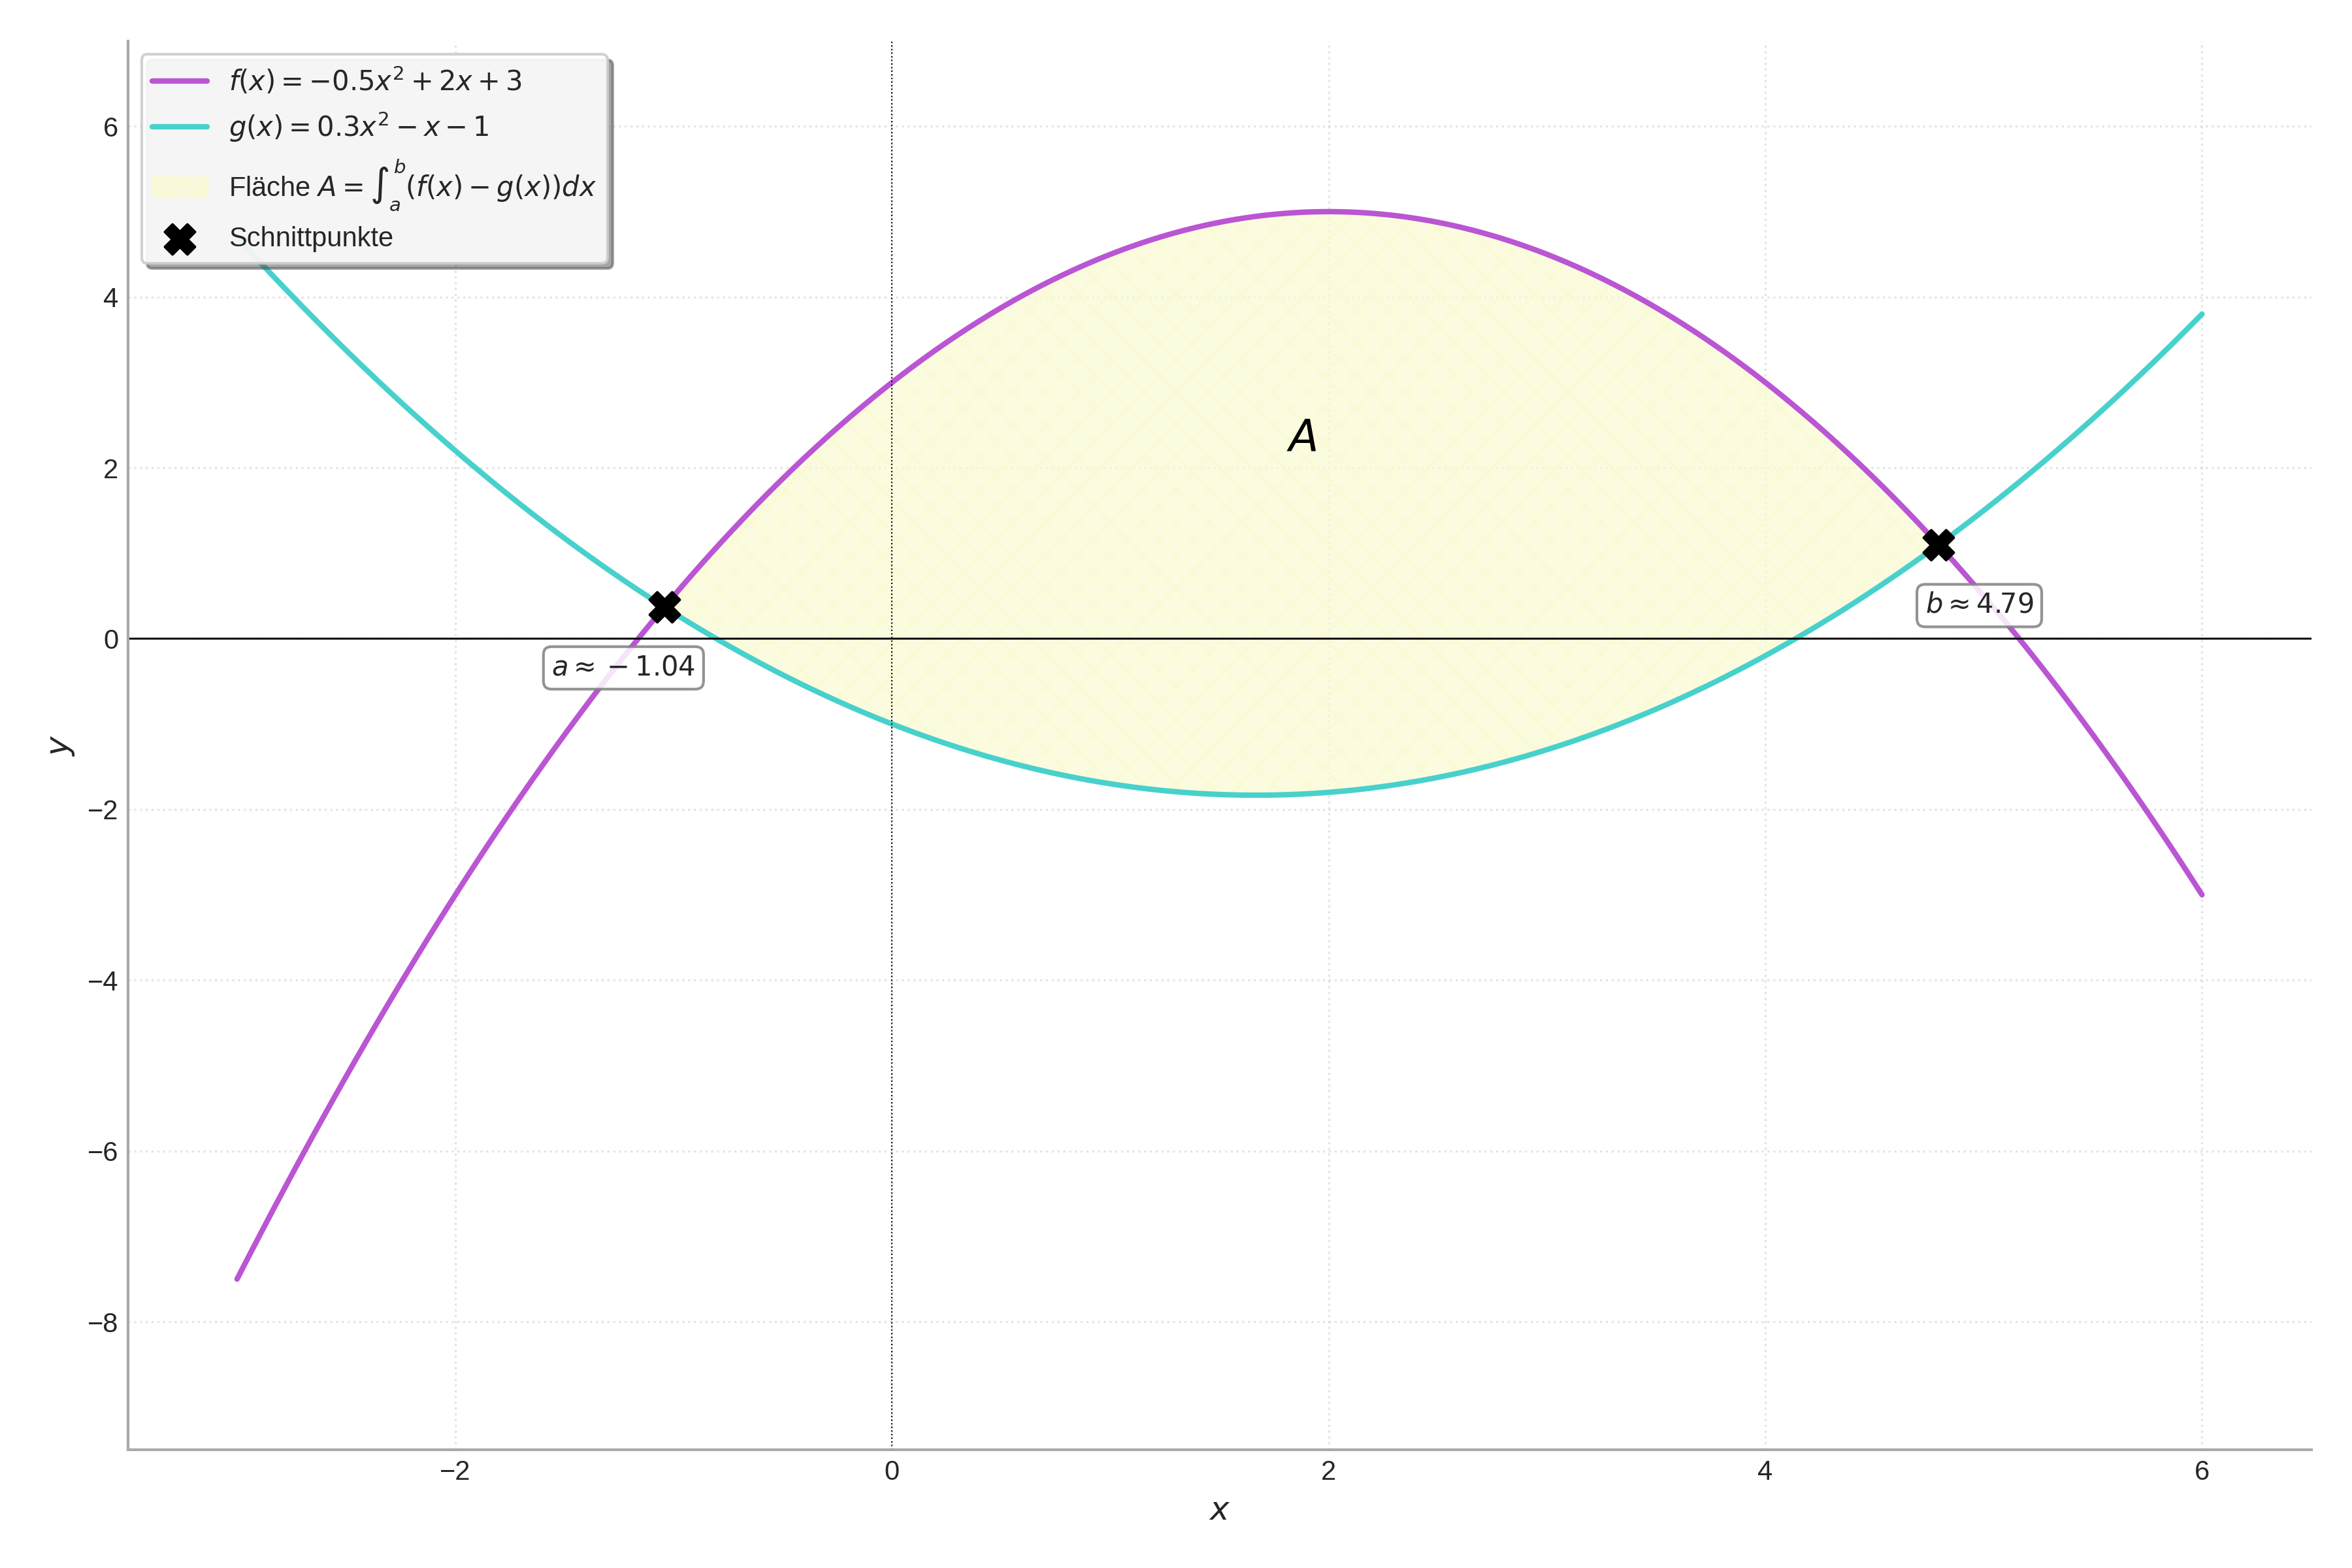
\includegraphics[width=0.8\textwidth]{grafiken/Integral_Flaeche_zwischen_Kurven.png}
    \captionof{figure}{Fläche zwischen den Graphen von $f(x)$ und $g(x)$}
    \label{fig:flaeche_zwischen_kurven}
\end{center}
\end{aufgabenumgebung}

\begin{aufgabenumgebung}{Der Mittelwert einer Funktion}
Manchmal möchte man nicht den Gesamtwert (wie die Gesamtfläche oder den Gesamtweg), sondern einen Durchschnittswert einer Größe über ein Intervall bestimmen. Die Integralrechnung hilft auch hier!

\begin{merksatzumgebung}{Mittelwert einer Funktion}
Der \textbf{Mittelwert $\mu$} einer stetigen Funktion $f(x)$ im Intervall $[a,b]$ (mit $a<b$) ist definiert als:
\[ \mu = \frac{1}{b-a} \int_a^b f(x) \,dx \]
\textit{Anschauliche Deutung:} Der Mittelwert $\mu$ ist die Höhe eines Rechtecks mit der Breite $(b-a)$, dessen Flächeninhalt gleich dem Flächeninhalt unter dem Graphen von $f(x)$ im Intervall $[a,b]$ ist. Also: $\mu \cdot (b-a) = \int_a^b f(x) \,dx$.
\end{merksatzumgebung}

\textbf{Aufgabe:}
Ein Tag hat vereinfacht 12 Stunden Helligkeit (von $t=0$ bis $t=12$). Die Temperatur $T$ (in °C) an diesem Tag kann durch die Funktion $T(t) = -0.5t^2 + 6t + 5$ modelliert werden.
\begin{enumerate}
    \item Skizziere den Graphen der Temperaturfunktion im Intervall $[0,12]$.
    \item Berechne die Durchschnittstemperatur während dieser 12 Stunden mit der Formel für den Mittelwert einer Funktion.
    \item Zeichne in deine Skizze ein Rechteck mit der Breite des Intervalls (12 Stunden) und der Höhe der Durchschnittstemperatur. Vergleiche die Fläche dieses Rechtecks mit der Fläche unter dem Temperatur-Graphen (visuell).
\end{enumerate}
\begin{center}
    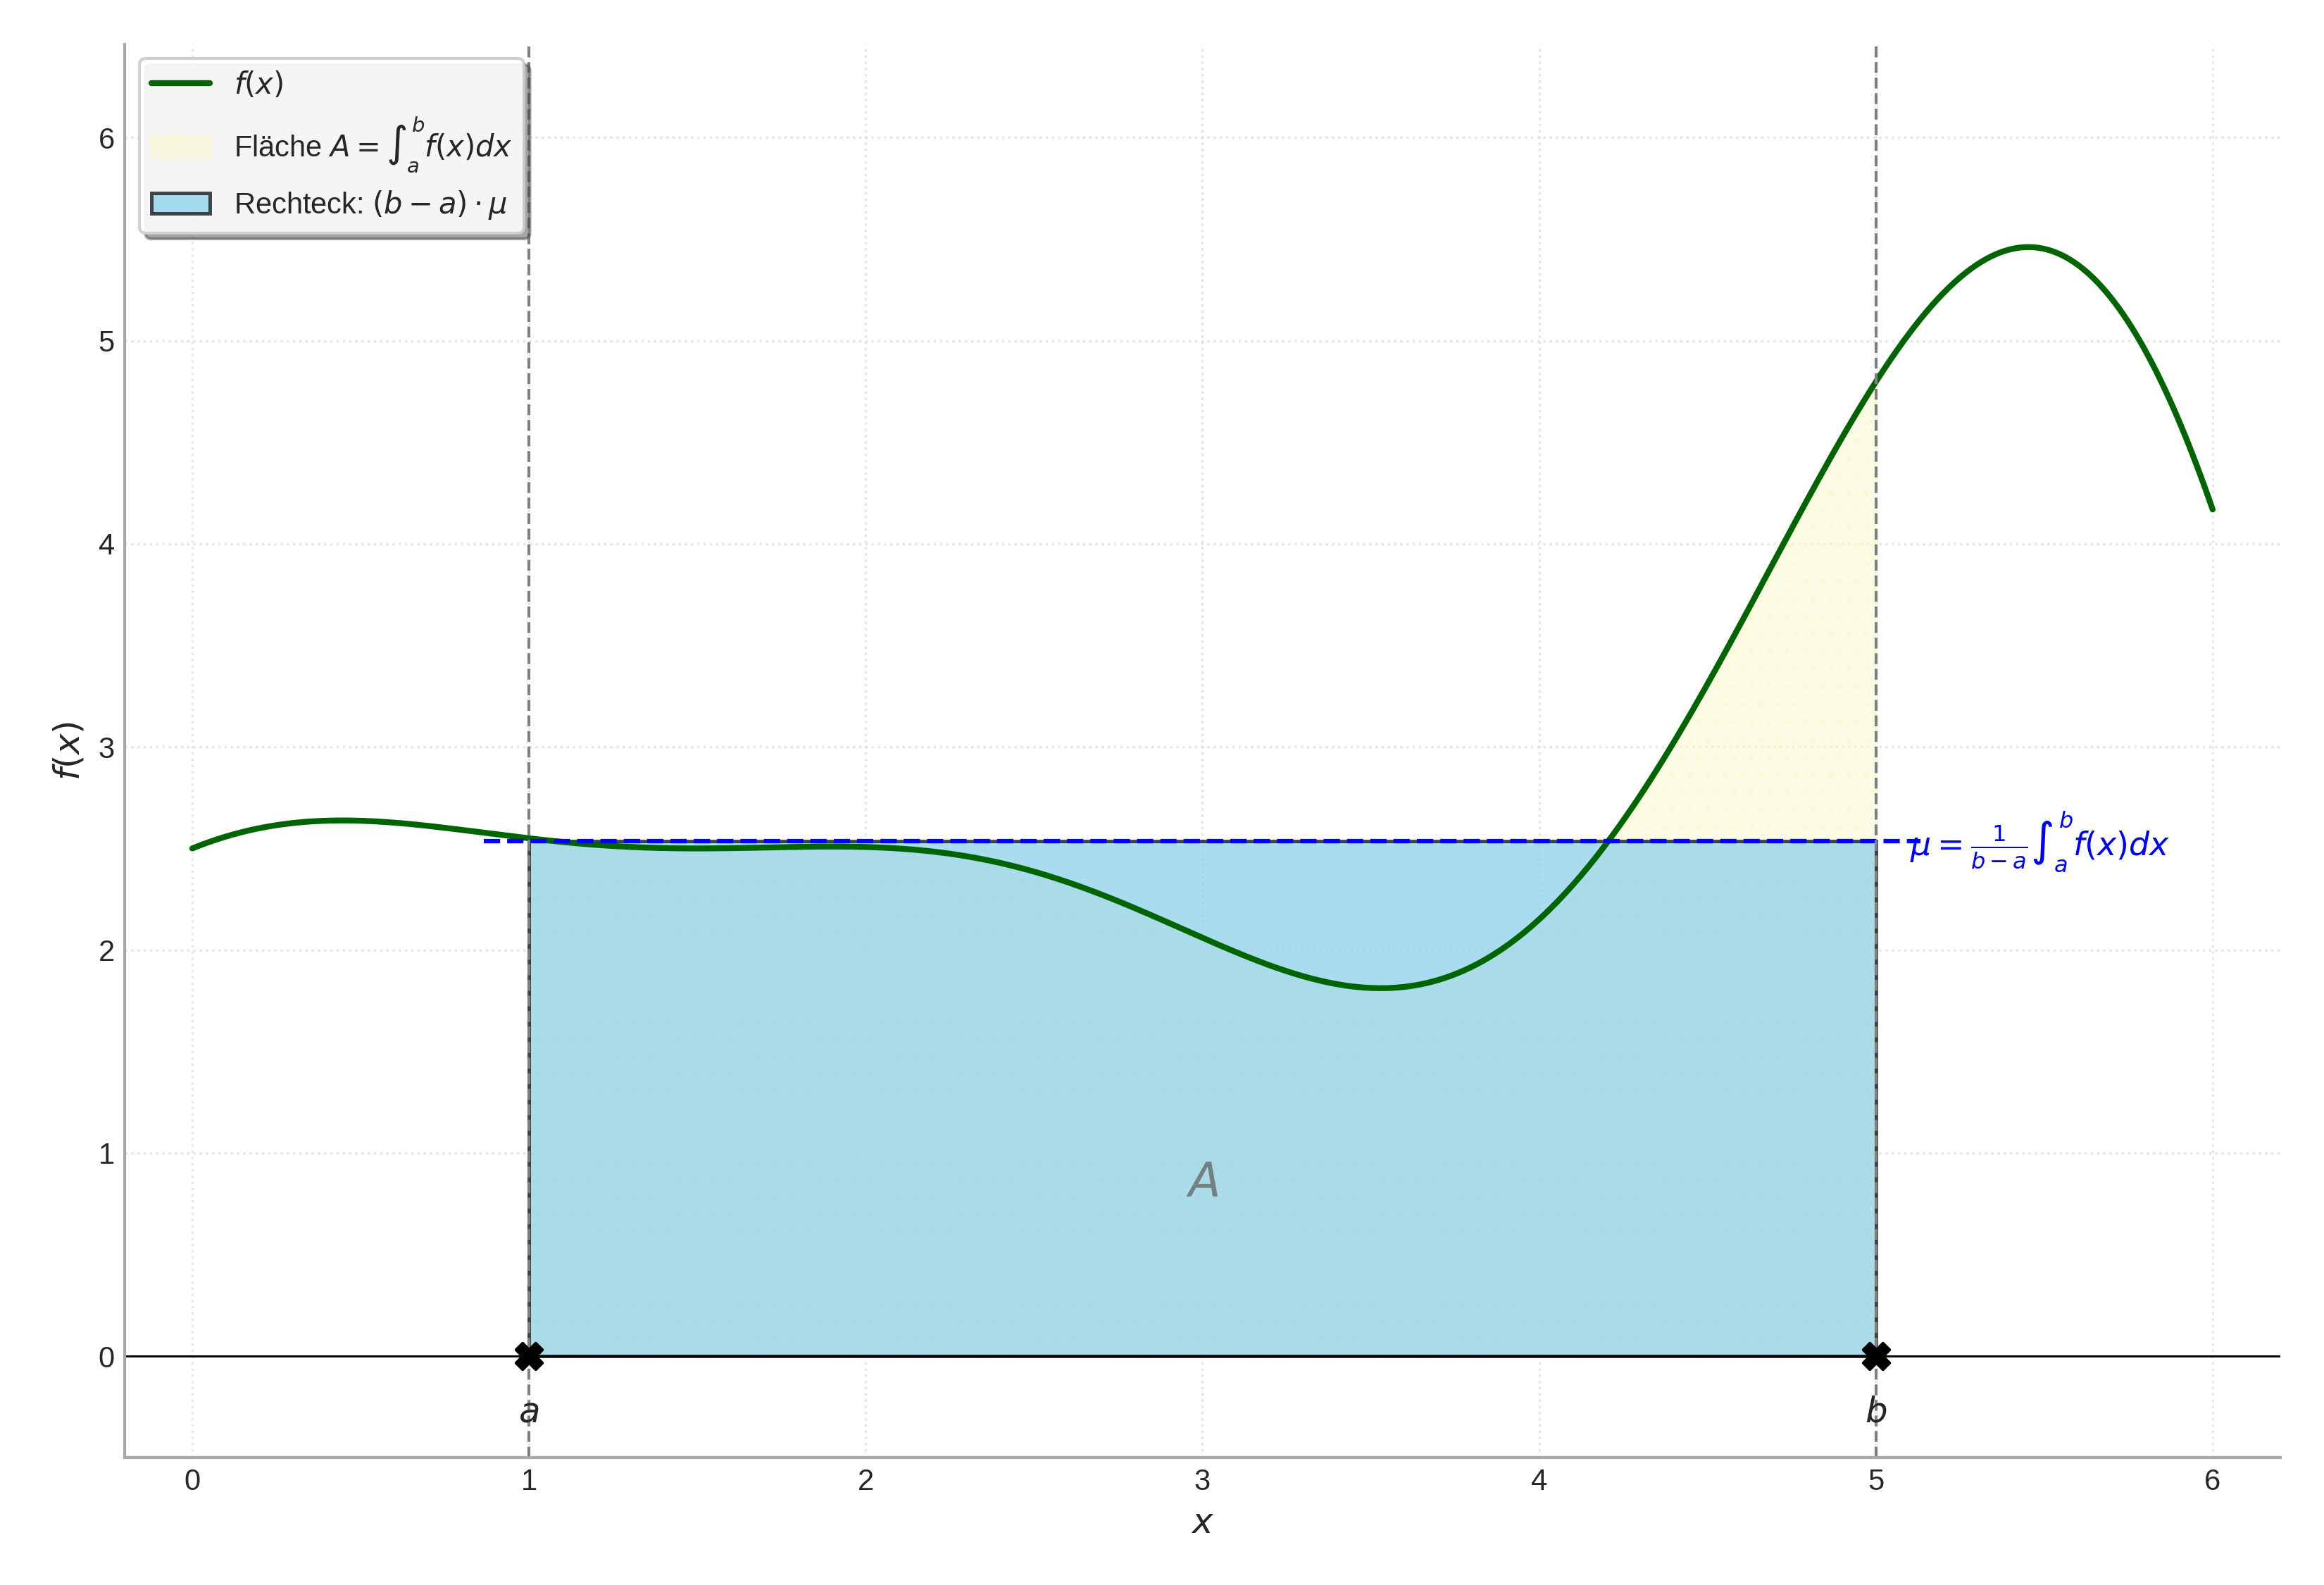
\includegraphics[width=0.8\textwidth]{grafiken/Integral_Mittelwert_Funktion.png}
    \captionof{figure}{Geometrische Deutung des Mittelwerts einer Funktion}
    \label{fig:mittelwert_funktion}
\end{center}
\end{aufgabenumgebung}

\begin{kurzknappumgebung}{Bestimmtes Integral und Hauptsatz}
\begin{itemize}
    \item \textbf{Bestimmtes Integral $\int_a^b f(x)dx$:} Grenzwert der Riemannsummen; gibt den orientierten Flächeninhalt zwischen Graph von $f(x)$ und x-Achse im Intervall $[a,b]$ an.
    \item \textbf{Stammfunktion $F(x)$:} Eine Funktion, deren Ableitung $f(x)$ ist ($F'(x)=f(x)$). Es gibt unendlich viele, die sich durch eine Konstante $C$ unterscheiden: $\int f(x)dx = F(x)+C$ (unbestimmtes Integral).
    \item \textbf{Hauptsatz (HDI):} $\int_a^b f(x)dx = F(b) - F(a)$. Ermöglicht einfache Berechnung bestimmter Integrale über Stammfunktionen.
    \item \textbf{Flächenberechnung:} Bei Nullstellen im Intervall müssen Teilintegrale gebildet und Beträge addiert werden für den geometrischen Flächeninhalt.
    \item \textbf{Symmetrie nutzen:} Bei punktsymmetrischen Funktionen über $[-a,a]$ ist $\int_{-a}^a f(x)dx = 0$. Bei achsensymmetrischen ist $\int_{-a}^a f(x)dx = 2 \cdot \int_0^a f(x)dx$.
    \item \textbf{Fläche zwischen Kurven $f(x)$ und $g(x)$ (mit $f(x) \ge g(x)$):} $A = \int_a^b (f(x)-g(x))dx$.
    \item \textbf{Mittelwert $\mu$ von $f(x)$ auf $[a,b]$:} $\mu = \frac{1}{b-a}\int_a^b f(x)dx$.
\end{itemize}
\end{kurzknappumgebung}

% Vorheriger Inhalt des Kapitels bis zur aufgabenumgebung 'Der Mittelwert einer Funktion'
% ... (siehe vorherige Canvas-Version) ...

\subsection{Zusammenfassung und Ausblick zur Integralrechnung}
\label{subsec:zusammenfassung_ausblick_integral}

Wir haben nun die fundamentalen Ideen der Integralrechnung kennengelernt: von der anschaulichen Flächenapproximation durch Riemannsummen über das Konzept der Stammfunktion als 'Gegenstück' zur Ableitung bis hin zum mächtigen Hauptsatz der Differential- und Integralrechnung. Mit diesen Werkzeugen können wir bereits viele wichtige Probleme lösen, insbesondere Flächeninhalte unter und zwischen Kurven von Polynomfunktionen berechnen sowie Mittelwerte von Funktionen bestimmen.

\begin{kurzknappumgebung}{Integralrechnung – Das Wichtigste auf einen Blick}
\begin{itemize}
    \item \textbf{Riemannsummen (Unter-/Obersumme):} Annäherung von Flächen unter Kurven durch Summen von Rechtecksflächen.
    \item \textbf{Bestimmtes Integral $\int_a^b f(x)dx$:} Grenzwert der Riemannsummen; gibt den orientierten Flächeninhalt zwischen dem Graphen von $f(x)$ und der x-Achse im Intervall $[a,b]$ an.
    \item \textbf{Stammfunktion $F(x)$:} Eine Funktion, deren Ableitung $f(x)$ ist ($F'(x)=f(x)$). Es gibt unendlich viele Stammfunktionen, die sich durch eine additive Konstante $C$ unterscheiden: $\int f(x)dx = F(x)+C$ (unbestimmtes Integral).
    \item \textbf{Hauptsatz der Differential- und Integralrechnung (HDI):} Die Brücke zwischen Ableiten und Integrieren!
    \[ \int_a^b f(x)dx = [F(x)]_a^b = F(b) - F(a) \]
    Er ermöglicht die exakte Berechnung bestimmter Integrale über Stammfunktionen.
    \item \textbf{Flächenberechnung:}
        \begin{itemize}
            \item Liegt $f(x)$ im Intervall $[a,b]$ nicht unterhalb der x-Achse, ist $A = \int_a^b f(x)dx$.
            \item Bei Nullstellen im Intervall müssen Teilintegrale gebildet und deren Beträge addiert werden, um den geometrischen Gesamtflächeninhalt zu erhalten ($A = \int_a^b |f(x)|dx$).
            \item Fläche zwischen zwei Kurven $f(x)$ und $g(x)$ (mit $f(x) \ge g(x)$ auf $[a,b]$): $A = \int_a^b (f(x)-g(x))dx$.
        \end{itemize}
    \item \textbf{Symmetrie nutzen:} Bei punktsymmetrischen Funktionen über $[-a,a]$ ist $\int_{-a}^a f(x)dx = 0$. Bei achsensymmetrischen ist $\int_{-a}^a f(x)dx = 2 \cdot \int_0^a f(x)dx$.
    \item \textbf{Mittelwert $\mu$ von $f(x)$ auf $[a,b]$:} $\mu = \frac{1}{b-a}\int_a^b f(x)dx$.
\end{itemize}
\end{kurzknappumgebung}

\begin{infoboxumgebung}{Ausblick: Was kommt noch in der Integralrechnung?}
Die bisher gelernten Integrationsregeln (Potenz-, Faktor-, Summenregel als Umkehrung der Ableitungsregeln) reichen für Polynomfunktionen und einfache gebrochen-rationale Funktionen gut aus. Aber was ist mit komplexeren Funktionen, die wir bereits beim Ableiten kennengelernt haben?
\begin{itemize}
    \item Wie integriert man Produkte von Funktionen, z.B. $f(x) = x^2 \cdot e^x$?
    \item Wie integriert man Quotienten, z.B. $g(x) = \frac{2x}{x^2+1}$?
    \item Wie integriert man verkettete Funktionen, z.B. $h(x) = (3x+5)^4$ oder $k(x) = e^{x^2+x+1} \cdot (2x+1)$ oder $m(x) = x \cdot \sin(x^2)$?
\end{itemize}
Für solche Fälle gibt es weiterführende \textbf{Integrationstechniken}, die oft auf der Umkehrung der komplexeren Ableitungsregeln basieren:
\begin{itemize}
    \item Die \textbf{partielle Integration} (Umkehrung der Produktregel).
    \item Die \textbf{Integration durch Substitution} (Umkehrung der Kettenregel).
    % \item Die \textbf{Partialbruchzerlegung} für kompliziertere gebrochen-rationale Funktionen.
\end{itemize}
Diese Techniken erweitern unseren 'Integrations-Werkzeugkasten' erheblich und ermöglichen die Behandlung einer viel größeren Klasse von Funktionen. Sie sind oft Gegenstand weiterführender Kurse oder Vertiefungen in der Oberstufe.

Auch das Integrieren von Exponentialfunktionen (wie $e^x$), Logarithmusfunktionen (wie $\ln x$) und trigonometrischen Funktionen (wie $\sin x, \cos x$) erfordert eigene Stammfunktionen, die du noch kennenlernen wirst. Die Welt der Integrale ist groß und mächtig! Das Fundament, das du hier gelegt hast, ist aber entscheidend für alles Weitere.
\end{infoboxumgebung}



\begin{aufgabenumgebung}{Checkliste: Das bestimmte Integral – Von der Summe zur Fläche}
Das bestimmte Integral ist ein zentrales Konzept der Analysis. Diese Fragen helfen dir, die Idee dahinter besser zu greifen:

\begin{enumerate}[label=(\alph*)]
    \item \textbf{Riemannsummen als Annäherung:}
    \begin{itemize}
        \item Erkläre mit eigenen Worten, warum die Unter- und Obersumme sich dem tatsächlichen Flächeninhalt unter einer Kurve annähern, wenn man die Anzahl $n$ der Rechtecke immer weiter erhöht. Was passiert dabei mit der Breite $\Delta x$ der einzelnen Rechtecke?
        \item Skizziere eine Funktion, die in einem Intervall $[a,b]$ sowohl positive als auch negative Werte annimmt. Wie würdest du die Riemannsumme (z.B. mit linken Rändern) interpretieren? Was passiert mit den Rechtecksflächen, die unterhalb der x-Achse liegen?
    \end{itemize}
    \item \textbf{Das bestimmte Integral $\int_a^b f(x)dx$:}
    \begin{itemize}
        \item Was bedeuten die einzelnen Bestandteile der Notation: $\int$, $a$, $b$, $f(x)$ und $dx$? Welche Rolle spielt das $dx$ in Erinnerung an die Riemannsummen?
        \item Wenn $f(x)$ die Änderungsrate einer Größe beschreibt (z.B. die Geschwindigkeit $v(t)$ in m/s), welche Bedeutung und welche Einheit hat dann das bestimmte Integral $\int_{t_1}^{t_2} f(x)dx$ (bzw. $\int_{t_1}^{t_2} v(t)dt$)?
    \end{itemize}
    \item \textbf{Orientierte Fläche vs. Geometrische Fläche:}
    \begin{itemize}
        \item Angenommen, $\int_0^2 f(x)dx = 5$ und $\int_2^3 f(x)dx = -2$. Was ist der Wert von $\int_0^3 f(x)dx$? Welchen geometrischen Gesamtflächeninhalt schließt der Graph von $f(x)$ mit der x-Achse im Intervall $[0,3]$ ein? Erkläre den Unterschied.
        \item Wie würdest du vorgehen, um den \textit{geometrischen} Flächeninhalt zwischen dem Graphen von $f(x)=x^3-x$ und der x-Achse im Intervall $[-1,1]$ zu berechnen? Warum reicht hier nicht einfach $\int_{-1}^1 (x^3-x)dx$? (Tipp: Symmetrie und Nullstellen beachten).
    \end{itemize}
    \item \textbf{Eigenschaften des bestimmten Integrals:}
    \begin{itemize}
        \item Was ist der Wert von $\int_a^a f(x)dx$ und warum?
        \item Welcher Zusammenhang besteht zwischen $\int_a^b f(x)dx$ und $\int_b^a f(x)dx$? Wie lässt sich das mit $F(b)-F(a)$ erklären?
    \end{itemize}
\end{enumerate}
\end{aufgabenumgebung}

\begin{aufgabenumgebung}{Checkliste: Stammfunktion und Hauptsatz – Die große Verbindung}
Die Entdeckung des Zusammenhangs zwischen Ableitung und Integral durch den Hauptsatz ist revolutionär. Teste dein Verständnis:

\begin{enumerate}[label=(\alph*)]
    \item \textbf{Stammfunktion und unbestimmtes Integral:}
    \begin{itemize}
        \item Erkläre den Unterschied zwischen 'einer Stammfunktion $F(x)$ von $f(x)$' und 'dem unbestimmten Integral $\int f(x)dx$'. Warum ist die Integrationskonstante $C$ beim unbestimmten Integral so wichtig?
        \item Wenn $F(x)$ eine Stammfunktion von $f(x)$ ist und $G(x)$ eine Stammfunktion von $g(x)$ ist: Ist $F(x) \cdot G(x)$ dann automatisch eine Stammfunktion von $f(x) \cdot g(x)$? Überprüfe deine Vermutung mit einem einfachen Beispiel (z.B. $f(x)=1, g(x)=2x$). Was schließt du daraus für Integrationsregeln für Produkte?
    \end{itemize}
    \item \textbf{Der Hauptsatz der Differential- und Integralrechnung (HDI):}
    \begin{itemize}
        \item Formuliere den HDI mit eigenen Worten. Was ist die 'Brücke', die er zwischen der Differential- und Integralrechnung schlägt?
        \item Warum ist der HDI so praktisch für die Berechnung von bestimmten Integralen im Vergleich zur Methode mit den Riemannsummen?
        \item Angenommen, jemand behauptet, eine Stammfunktion von $f(x)=2x$ sei $F(x)=x^2+1000$, und eine andere Person sagt, es sei $G(x)=x^2-5$. Wer hat Recht? Und wie wirkt sich die Wahl von $F(x)$ oder $G(x)$ auf das Ergebnis von $\int_1^2 2x \,dx$ aus? Begründe.
    \end{itemize}
    \item \textbf{Anwendungen und Interpretationen:}
    \begin{itemize}
        \item Wenn $\int_a^b f(x)dx = 0$ ist, bedeutet das zwangsläufig, dass $f(x)=0$ für alle $x \in [a,b]$ gilt? Erkläre anhand einer Skizze oder eines Beispiels (nutze Symmetrie!).
        \item Erkläre die geometrische Bedeutung des Mittelwerts $\mu = \frac{1}{b-a} \int_a^b f(x)dx$ einer Funktion $f(x)$ im Intervall $[a,b]$ mithilfe eines flächengleichen Rechtecks.
    \end{itemize}
\end{enumerate}
\end{aufgabenumgebung}



